\documentclass[11pt,a4paper]{article}

% ── Packages ──────────────────────────────────────────────────────────────────
\usepackage[margin=2.5cm]{geometry}
\usepackage{amsmath,amssymb,amsthm}
\usepackage{graphicx}
\usepackage[labelfont=bf,font=small,skip=6pt]{caption}
\usepackage[font=small]{subcaption}
\usepackage{booktabs}
\usepackage{array}
\usepackage{xcolor}
\usepackage{hyperref}
\usepackage{microtype}
\usepackage{float}
\usepackage{algorithm}
\usepackage{algpseudocode}
\usepackage{listings}
\usepackage{enumitem}
\usepackage{nicefrac}
\usepackage{multirow}
\usepackage{tikz}
\usetikzlibrary{arrows.meta, shapes.geometric, positioning, calc}

% ── Hyperref setup ─────────────────────────────────────────────────────────────
\hypersetup{
  colorlinks=true,
  linkcolor=blue!70!black,
  citecolor=green!50!black,
  urlcolor=cyan!70!black,
}

% ── Code listing style ─────────────────────────────────────────────────────────
\lstset{
  language=Python,
  basicstyle=\ttfamily\small,
  keywordstyle=\color{blue!70!black}\bfseries,
  commentstyle=\color{green!50!black}\itshape,
  stringstyle=\color{red!70!black},
  frame=single,
  rulecolor=\color{gray!40},
  breaklines=true,
  breakatwhitespace=true,
  tabsize=4,
  showstringspaces=false,
}

% ── Math operators and notation ────────────────────────────────────────────────
\DeclareMathOperator{\sigmoid}{sigmoid}
\DeclareMathOperator{\atanh}{atanh}
\DeclareMathOperator*{\argmin}{arg\,min}
\newcommand{\W}{\mathbf{W}}
\newcommand{\Wraw}{\tilde{\mathbf{W}}}
\newcommand{\I}{\mathbf{I}}
\newcommand{\R}{\mathbb{R}}
\newcommand{\Render}{\mathcal{R}}
\newcommand{\MSE}{\mathrm{MSE}}
\newcommand{\PSNR}{\mathrm{PSNR}}

% ── Table of contents depth ────────────────────────────────────────────────────
\setcounter{tocdepth}{2}

% ─────────────────────────────────────────────────────────────────────────────
\begin{document}

\begin{titlepage}
  \centering
  \vspace*{2cm}

  {\LARGE\bfseries Gaussian Encoder Validation Report}\\[0.6em]
  {\large Architecture, Bug Discovery, and Readiness for\\
   Diffusion Model Training}\\[3em]

  {\large Sander Coessens$^{1}$ \quad Aryan Samal$^{1}$ \quad
          Anshul Malhotra$^{1}$ \quad Naila Seghouani$^{1}$}\\[0.5em]
  {\normalsize $^{1}$CentraleSupélec, Université Paris-Saclay}\\[3em]

  {\large March 2026}\\[2em]

  \begin{abstract}
    We present a comprehensive validation study of the \emph{Gaussian encoder} used in
GaussianDiffusion, a diffusion model that operates in the latent space of 2-D Gaussian
splatting representations.  The encoder fits $K$ two-dimensional Gaussians to a greyscale
image by gradient descent, producing a compact $K\!\times\!7$ parameter tensor that
a downstream DDPM transformer subsequently learns to generate.

During development a critical \textbf{coordinate-inversion bug} was discovered: the
renderer (\texttt{F.affine\_grid}) inverts the translation coordinates, causing
Gaussian seeds placed at pixel positions $(x, y)$ to render on the opposite side of
the image.  Prior to the fix the encoder achieved only $26\,\mathrm{dB}$ mean PSNR
with $60\%$ dead Gaussians even after $3\,000$ epochs.  Three one-line changes to
the initialisation, dead-mask, and recycling routines corrected the convention, raising
mean PSNR to $\mathbf{44.2 \pm 3.7\,\mathrm{dB}}$ with $\mathbf{100\%}$ alive
Gaussians and convergence within ${\sim}790$ epochs on average.

We validate the encoder on MNIST across all ten digit classes, report per-digit PSNR
statistics, convergence dynamics, parameter distributions, spatial structure of the
learned Gaussians, K-sensitivity, and a loss-function ablation (MSE vs.\ L1\,+\,SSIM).
We further assess \emph{downstream readiness}: whether the encoded representations
are suitable as training data for a diffusion model, examining normalization coverage,
latent-space structure (PCA), encoding consistency, and the vestigial $\alpha$ parameter.
Our analysis confirms that the corrected encoder produces clean, normalizable, structurally
coherent representations that are ready for diffusion model training.

  \end{abstract}

  \vfill
  {\small
    \textbf{Code and data:}
    Project at \texttt{GaussianDiffusion/}.
    Figures generated by \texttt{reports/encoder\_research/generate\_figures.py}.
  }
\end{titlepage}

\tableofcontents
\newpage

% ── Main body ─────────────────────────────────────────────────────────────────
\section{Introduction}
\label{sec:introduction}

Generative models have made remarkable progress on pixel-space images, but the
computational cost of operating directly on dense pixel grids motivates the search
for compact latent representations.
\emph{Gaussian splatting}~\cite{kerbl20233d} provides one such representation:
an image is described as a superposition of $K$ anisotropic 2-D Gaussians,
each parameterised by position, scale, orientation, colour, and opacity.
Such representations are interpretable, differentiable, and naturally sparse.

The \textbf{GaussianDiffusion} project exploits Gaussian splatting as a latent
space for a denoising diffusion probabilistic model (DDPM).  The pipeline is:

\begin{enumerate}[leftmargin=2em]
  \item \textbf{Encode:} fit $K$ Gaussians to each training image using gradient
        descent $\rightarrow$ tensor $\W \in \R^{K \times 7}$.
  \item \textbf{Train:} learn a DDPM GaussianTransformer that generates $\W$
        tensors from Gaussian noise.
  \item \textbf{Sample:} run reverse diffusion on the transformer, then render
        the predicted $\W$ with the Gaussian splatting renderer to obtain images.
\end{enumerate}

\noindent
This report focuses exclusively on \textbf{Step~1}: the correctness, quality, and
downstream suitability of the encoder.
A sound encoder is a prerequisite for everything downstream.
Poor reconstructions set a hard ceiling on generative quality; parameter
distributions that violate assumptions (non-smooth, multi-modal, poorly normalised)
make diffusion training harder.

\subsection{Scope and Contributions}

\noindent This report makes the following contributions:

\begin{itemize}[leftmargin=2em]
  \item A full description of the encoder's architecture and optimisation procedure
        (\S\ref{sec:architecture}).
  \item A mathematical account of the Gaussian splatting renderer, including an
        explanation of the \texttt{F.affine\_grid} coordinate convention
        (\S\ref{sec:renderer}).
  \item Discovery and diagnosis of a coordinate-inversion bug that prevented
        convergence, and verification of the three-line fix (\S\ref{sec:bug}).
  \item Quantitative validation on MNIST: per-digit PSNR statistics, convergence
        dynamics, K-sensitivity, loss-function ablation, and parameter analysis
        (\S\ref{sec:experiments}).
  \item Assessment of downstream readiness for diffusion model training
        (\S\ref{sec:downstream}).
\end{itemize}

\subsection{Dataset and Setting}

All experiments use the MNIST handwritten-digit dataset
($28 \times 28$ greyscale images, pixel values in $[0,1]$).
We encode $N = 50$ images (5 per digit class) using the corrected encoder
with $K = 70$ Gaussians, $3{,}000$ maximum epochs, learning rate $5\!\times\!10^{-3}$,
kernel size $11$, and early stopping at MSE\,$ < 10^{-4}$ ($\approx 40\,\text{dB}$
PSNR).  Additional experiments vary $K$, the loss function, and the random seed.
All computations are performed on CPU; the same code runs on GPU without modification.

\section{Encoder Architecture}
\label{sec:architecture}

\subsection{Optimisation Objective}

Given a greyscale target image $\I \in [0,1]^{H \times W}$, the encoder finds
physical Gaussian parameters $\W^* \in \R^{K \times 7}$ that minimise
mean-squared error (MSE) between the rendered image and the target:

\begin{equation}
  \W^* = \argmin_{\W} \;\MSE\!\bigl(\Render(\W),\, \I\bigr)
       = \argmin_{\W} \;\frac{1}{HW}\sum_{i,j}
         \bigl(\Render(\W)_{ij} - \I_{ij}\bigr)^2,
  \label{eq:objective}
\end{equation}

\noindent where $\Render(\W)$ is the differentiable Gaussian splatting renderer
(Section~\ref{sec:renderer}).

\subsection{Parameter Layout}

Each Gaussian $k \in \{1,\ldots,K\}$ is described by a 7-dimensional parameter
vector $\W_{k,:} = [\sigma_x,\, \sigma_y,\, \rho,\, \alpha,\, c,\, x,\, y]$
with the physical ranges shown in Table~\ref{tab:params}.

\begin{table}[ht]
\centering
\caption{Physical parameters of each 2-D Gaussian (one row of $\W$).}
\label{tab:params}
\begin{tabular}{lllp{6.5cm}}
\toprule
\textbf{Symbol} & \textbf{Name} & \textbf{Range} & \textbf{Meaning} \\
\midrule
$\sigma_x$ & std.\ dev.\ $x$ & $(0, 1)$  & Horizontal spread of the Gaussian \\
$\sigma_y$ & std.\ dev.\ $y$ & $(0, 1)$  & Vertical spread of the Gaussian \\
$\rho$     & correlation     & $(-1, 1)$ & Off-axis tilt; covariance $= \rho\sigma_x\sigma_y$ \\
$\alpha$   & opacity         & $(0, 1)$  & \emph{Vestigial} — not passed to renderer (§\ref{sec:alpha}) \\
$c$        & colour          & $(0, 1)$  & Greyscale intensity contributed by this Gaussian \\
$x$        & position $x$    & $(-1, 1)$ & Horizontal centre in normalised image coords \\
$y$        & position $y$    & $(-1, 1)$ & Vertical centre in normalised image coords \\
\bottomrule
\end{tabular}
\end{table}

\subsection{Raw Parameterisation and Differentiable Transforms}

The optimiser operates on \emph{unconstrained raw parameters}
$\Wraw \in \R^{K \times 7}$, mapped to physical space by smooth, bounded
transforms that maintain differentiability throughout:

\begin{align}
  \sigma_x &= \sigmoid(\Wraw_{:,0}), &
  \sigma_y &= \sigmoid(\Wraw_{:,1}), \label{eq:sigma}\\
  \rho     &= \tanh(\Wraw_{:,2}),    &
  \alpha   &= \sigmoid(\Wraw_{:,3}), \label{eq:rho}\\
  c        &= \sigmoid(\Wraw_{:,4}), &
  x        &= \tanh(\Wraw_{:,5}),\quad
  y = \tanh(\Wraw_{:,6}).              \label{eq:xy}
\end{align}

\noindent This reparameterisation ensures that gradient descent on $\Wraw$
cannot push any parameter outside its valid range, eliminating the need for
projected gradient methods or explicit clipping during training.

\subsection{Initialisation}
\label{sec:init}

Initialisation has a large impact on convergence speed.
Gradient descent on the rendering objective has many local minima, and
Gaussians that start far from bright image regions converge slowly or not at all.

\paragraph{Brightness-weighted seeding.}
We seed position $(x_k, y_k)$ by sampling pixel coordinates from the
distribution $p_\text{pixel} \propto \I_{ij}$ with replacement.
This concentrates initial Gaussians in bright (ink) regions where they must
contribute, rather than in background regions where their gradient signal is
near-zero.

\medskip\noindent
\textbf{Why with replacement?}\ \ Sampling without replacement spreads Gaussians
to dimmer pixels where the MSE gradient is weaker.
Competitive pressure from overlapping Gaussians — when several are seeded on
the same bright stroke — drives rapid spatial diversification in the first
${\sim}500$ epochs via gradient-driven competition, achieving ${\approx}6\,\text{dB}$
higher PSNR by epoch $1{,}000$ than without-replacement seeding.

\paragraph{Coordinate inversion convention.}
Due to the affine-grid coordinate inversion of the renderer
(Section~\ref{sec:coord_convention}), the initialisation must set
$\Wraw_{k,5} = \atanh(-x_\text{pixel})$ and
$\Wraw_{k,6} = \atanh(-y_\text{pixel})$
so that the Gaussian renders at the desired pixel position.
This was the source of the coordinate-inversion bug (Section~\ref{sec:bug}).

\paragraph{Shape initialisation.}
All $K$ Gaussians are initialised with equal, small radii:
$\Wraw_{k,0} = \Wraw_{k,1} = -1.5$ (i.e.\ $\sigma_x = \sigma_y \approx 0.18$),
zero correlation ($\Wraw_{k,2} = 0$), and colour seeded from the pixel value
$c_k = \sigmoid(\logit(\I_{y_k, x_k}))$.

\paragraph{All-black images.}
If $\|\I\|_1 < 10^{-7}$ (all-black image), pixel-weighted sampling degenerates.
In this case positions are sampled uniformly, which is the correct behaviour.

\subsection{Optimisation}
\label{sec:optimisation}

We optimise $\Wraw$ with Adam and a cosine annealing schedule with warm restarts:

\begin{itemize}[leftmargin=2em]
  \item \textbf{Optimiser}: Adam, $\eta = 5 \times 10^{-3}$.
  \item \textbf{Scheduler}: CosineAnnealingWarmRestarts with $T_0 = \lfloor
        \text{epochs}/3 \rfloor$, $T_\text{mult} = 1$, $\eta_\text{min} = 10^{-5}$.
        Three full cosine cycles allow the learning rate to reset to its full value,
        helping the optimiser escape shallow local minima.
        Empirically, images that plateau at ${\sim}26\,\text{dB}$ can jump $6\text{--}9\,\text{dB}$
        when the LR resets to ${\approx}10^{-3}$.
  \item \textbf{Early stopping}: training halts when MSE\,$<10^{-4}$
        ($\PSNR \approx 40\,\text{dB}$).
  \item \textbf{Maximum epochs}: $3{,}000$.
\end{itemize}

Algorithm~\ref{alg:encode} gives the complete training procedure.

\begin{algorithm}[ht]
\caption{Gaussian encoder for a single image}
\label{alg:encode}
\begin{algorithmic}[1]
\Require Image $\I \in [0,1]^{H \times W}$, $K$, \textit{epochs}, $\eta$,
         \textit{early\_stop}, \textit{recycle\_every}
\State $\Wraw \leftarrow \textsc{InitGaussians}(\I, K)$
       \Comment{brightness-weighted, coord-inversion aware}
\State $\theta \leftarrow \textsc{Adam}([\Wraw],\; \eta)$
\State $\textit{scheduler} \leftarrow \textsc{CosineWarmRestarts}(\theta,\; T_0=\lfloor\textit{epochs}/3\rfloor)$
\For{$e = 0, 1, \ldots, \textit{epochs}-1$}
  \State $\W \leftarrow \textsc{ToPhysical}(\Wraw)$
  \State $\hat{\I} \leftarrow \Render(\W)$
         \Comment{differentiable Gaussian splatting}
  \State $\ell \leftarrow \MSE(\hat{\I}, \I)$
  \State Back-propagate $\ell$ and update $\Wraw$ via $\theta$
  \State Step scheduler
  \If{$(e+1) \bmod \textit{recycle\_every} = 0$}
    \State $\textsc{Recycle}(\Wraw, \I, \theta)$
           \Comment{teleport dead Gaussians to under-reconstructed regions}
  \EndIf
  \If{$\ell < \textit{early\_stop}$} \textbf{break} \EndIf
\EndFor
\State \Return $\textsc{ToPhysical}(\Wraw)$
\end{algorithmic}
\end{algorithm}

\subsection{Dead-Gaussian Detection and Recycling}
\label{sec:recycling}

A Gaussian is \emph{dead} when its centre lies on a background pixel
(target intensity $< 0.05$).  These Gaussians contribute nothing to the
reconstruction and waste optimiser capacity.

Every \textit{recycle\_every} epochs (default: $300$), we detect dead Gaussians
and \emph{teleport} them to under-reconstructed regions:

\begin{enumerate}[leftmargin=2em]
  \item Render the current approximation $\hat{\I}$.
  \item Compute residual $r = (\I - \hat{\I})_+ = \max(0,\;\I - \hat{\I})$.
  \item Sample new positions weighted by $r$ (regions the model is missing most).
  \item Re-initialise dead rows of $\Wraw$ with new positions and pixel colours.
  \item Reset the Adam moment tensors for recycled rows (stale second moments
        from the dead region would otherwise cause a large spurious update).
\end{enumerate}

\noindent
\textbf{Why not use colour threshold for death detection?}\ \
Overlapping Gaussians legitimately suppress each other's colour through
gradient-driven competition, so colour~$<0.05$ is a false positive.
Only the spatial criterion (centre on background) is used.

\subsection{The Vestigial \texorpdfstring{$\alpha$}{alpha} Parameter}
\label{sec:alpha}

The $\alpha$ (opacity) parameter is decoded from the raw parameters by
$\alpha = \sigmoid(\Wraw_{:,3})$, but it is \emph{never passed to the renderer}.
The function \texttt{generate\_2D\_gaussian\_splatting} does not accept an opacity
argument; Gaussian contributions are composited additively weighted only by $c$
(colour).
As a result, $\alpha$ is free to take any value during training without affecting
the rendered image.
This is verified experimentally in Section~\ref{sec:alpha_exp}.

\section{Gaussian Splatting Renderer}
\label{sec:renderer}

\subsection{Mathematical Formulation}

Each Gaussian $k$ is characterised by a covariance matrix

\begin{equation}
  \Sigma_k =
  \begin{pmatrix}
    \sigma_{x,k}^2 & \rho_k\,\sigma_{x,k}\sigma_{y,k} \\
    \rho_k\,\sigma_{x,k}\sigma_{y,k} & \sigma_{y,k}^2
  \end{pmatrix},
  \label{eq:covariance}
\end{equation}

\noindent which defines an unnormalised 2-D Gaussian kernel on a $[-5,5]^2$ grid:

\begin{equation}
  G_k(\mathbf{u}) = \exp\!\Bigl(-\tfrac{1}{2}\,\mathbf{u}^\top \Sigma_k^{-1} \mathbf{u}\Bigr),
  \quad \mathbf{u} \in [-5, 5]^2.
  \label{eq:kernel}
\end{equation}

The kernel is normalised to unit peak ($G_k \leftarrow G_k / \max G_k$),
padded to $H \times W$, then translated to position $(x_k, y_k)$ via an affine
transformation.  The final image is the additive composition:

\begin{equation}
  \hat{\I}_{ij} = \mathrm{clamp}\!\left(
    \sum_{k=1}^{K} c_k \cdot G_k^{(x_k,y_k)}(i,j),\; 0, 1
  \right),
  \label{eq:compositing}
\end{equation}

\noindent where $G_k^{(x_k,y_k)}$ denotes the translated kernel.

\subsection{Implementation Details}

The renderer is implemented in \texttt{src/utils/gaussian\_to\_image.py} using
PyTorch's \texttt{F.affine\_grid} and \texttt{F.grid\_sample} for the translation.
Important implementation notes:

\paragraph{Covariance inversion.}
We use \texttt{torch.linalg.inv} (replacing the deprecated \texttt{torch.inverse})
for numerically robust inversion.
If $\det(\Sigma_k) \leq 0$ (which can occur for extreme $\rho$ values), a small
$\epsilon = 10^{-6}$ is added to the diagonal to restore positive-definiteness.

\paragraph{Kernel maximum clamping.}
The normalisation divisor $\max_{\mathbf{u}} G_k(\mathbf{u})$ is clamped to
$\geq 10^{-8}$ to prevent division-by-zero on near-zero kernels.

\paragraph{Channel handling.}
The renderer supports $C$ channels (default $C=1$ for greyscale).
For MNIST we use $C=1$; the code extends to RGB without modification.

\subsection{Coordinate Convention}
\label{sec:coord_convention}

Understanding the coordinate convention of \texttt{F.affine\_grid} is critical.
The affine transformation is defined by a $2 \times 3$ matrix $\theta$:

\begin{equation}
  \theta =
  \begin{pmatrix}
    1 & 0 & t_x \\
    0 & 1 & t_y
  \end{pmatrix}.
  \label{eq:theta}
\end{equation}

\noindent PyTorch's \texttt{F.affine\_grid} with \texttt{align\_corners=True}
maps each \emph{output} pixel at normalised position $\mathbf{g}$ to an \emph{input}
sample position $\mathbf{s} = \mathbf{g} + \mathbf{t}$.
In other words, setting $t_x = c > 0$ means output pixel at $g_x = 0$ (centre)
samples the input at $s_x = c$, effectively \emph{shifting the content to the left}.

\medskip
\noindent
\textbf{Key consequence:} a Gaussian kernel centred at input $s_x = 0$ with
translation $t_x = c$ appears at \emph{output} position $g_x = -c$.
Equivalently, to render a Gaussian at output position $x_\text{render}$,
the translation parameter must satisfy $t_x = -x_\text{render}$,
so the coordinate stored in $\Wraw_{k,5}$ must be
\begin{equation}
  \Wraw_{k,5} = \atanh(-x_\text{pixel}),
  \label{eq:coord_fix}
\end{equation}
where $x_\text{pixel} \in [-1,1]$ is the desired normalised pixel position.
This convention is illustrated in Figure~\ref{fig:coord_inversion}.

\begin{figure}[htbp]
  \centering
  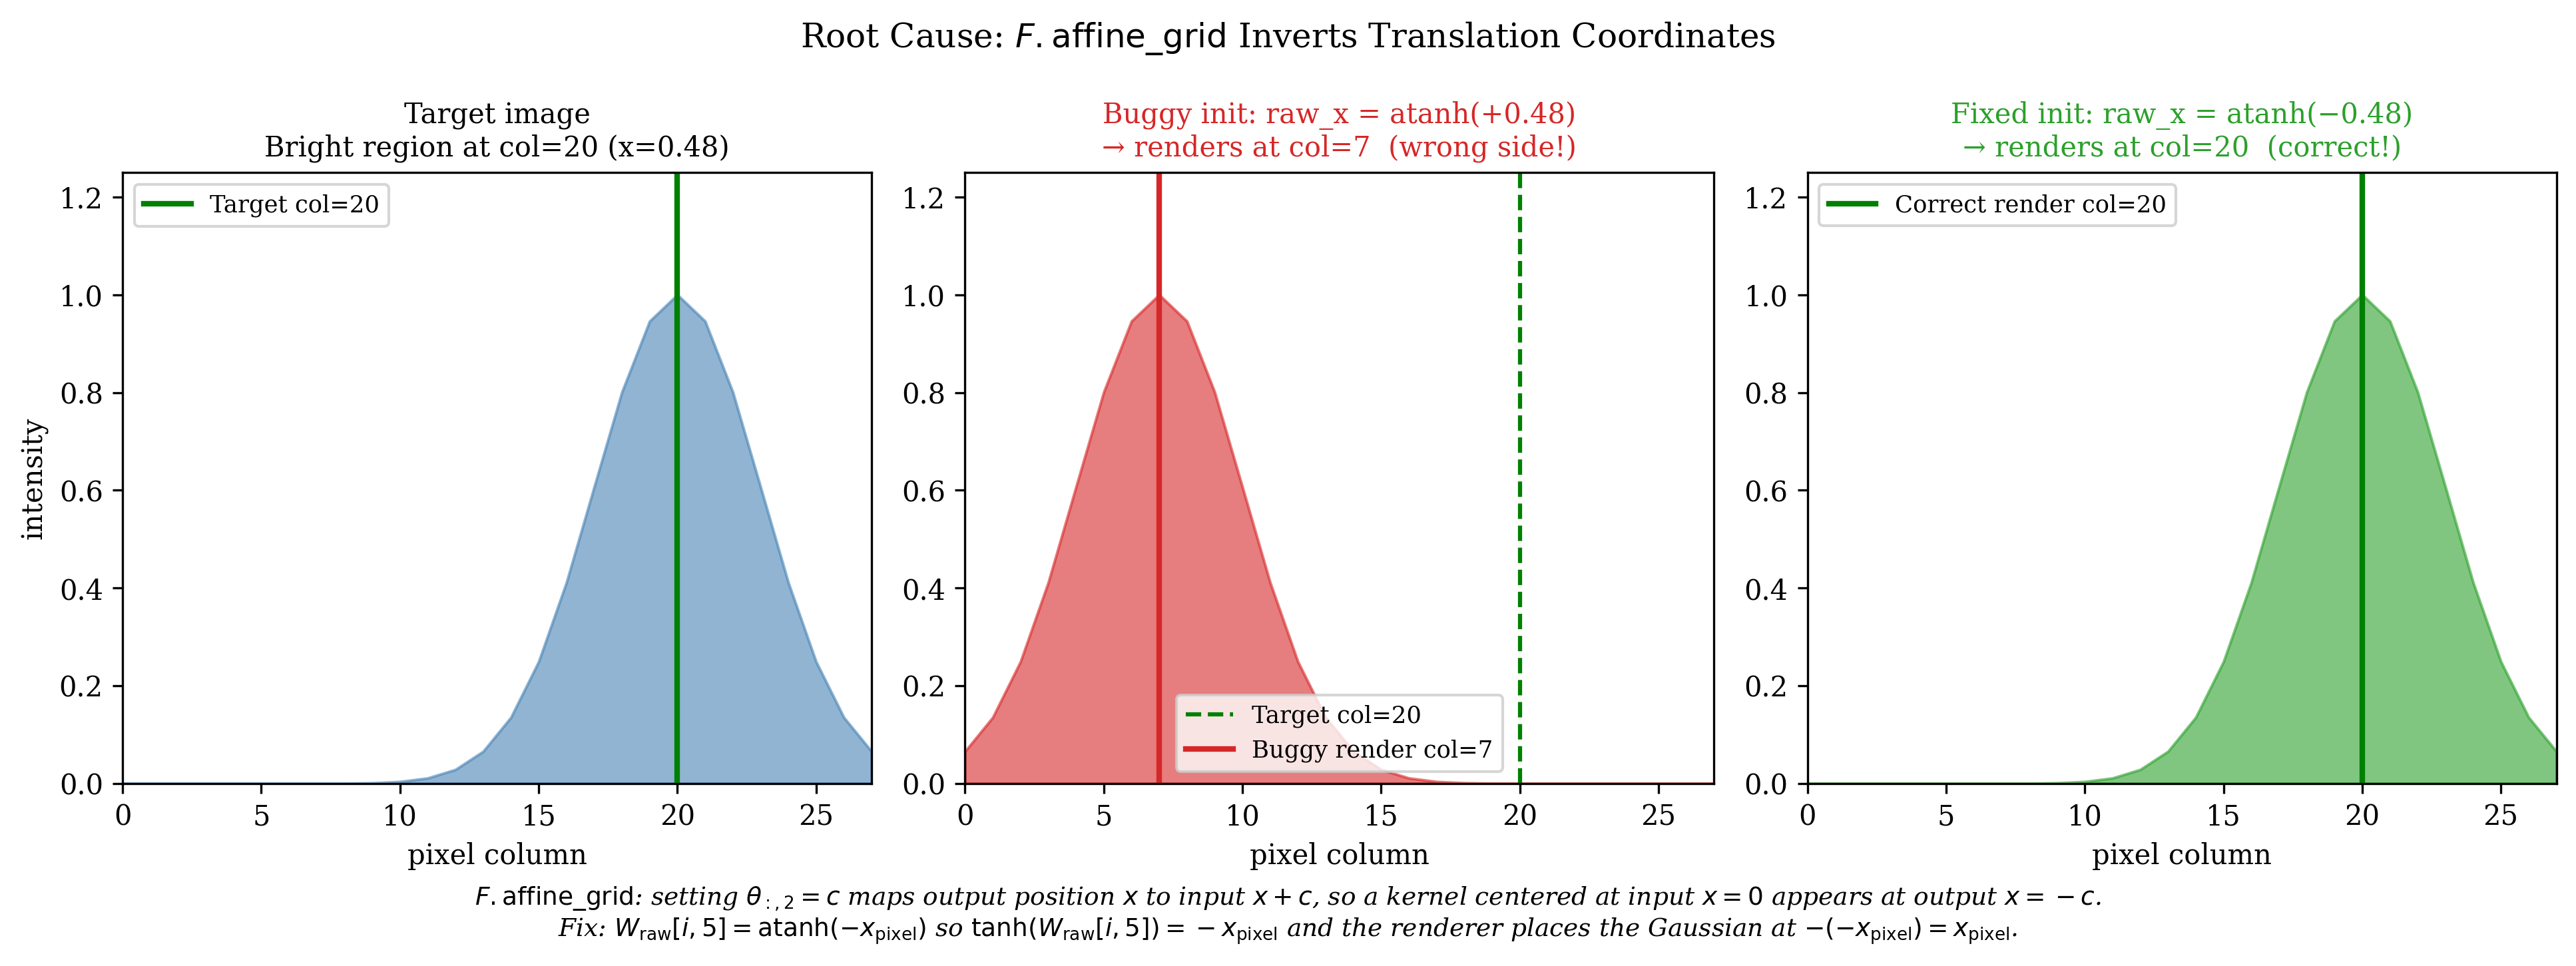
\includegraphics[width=\linewidth]{figures/fig_09_coord_inversion_diagram.png}
  \caption{%
    \textbf{Coordinate inversion in the renderer.}
    \emph{Left:} target image with a bright region at column~20 ($x \approx +0.48$).
    \emph{Centre:} with the buggy initialisation ($\Wraw_{k,5} = \atanh(+0.48)$),
    the Gaussian renders at column~$\approx 6$ (wrong side).
    \emph{Right:} with the corrected initialisation ($\Wraw_{k,5} = \atanh(-0.48)$),
    the Gaussian renders at column~20 (correct).
    The formula at the bottom summarises the \texttt{F.affine\_grid} convention.%
  }
  \label{fig:coord_inversion}
\end{figure}

\section{Bug Discovery and Fix}
\label{sec:bug}

\subsection{Symptom}

During initial development, the encoder was found to converge poorly on MNIST.
Even after $3{,}000$ epochs with $K = 70$ Gaussians, the best-case mean PSNR was
${\approx}26\,\text{dB}$, approximately $60\%$ of Gaussians were ``dead''
(centred on background pixels contributing nothing), and none of the images
reached the $40\,\text{dB}$ early-stop threshold.

\subsection{Root Cause Analysis}

\paragraph{Step 1: Identify the plateau.}
Monitoring the training loss revealed that the optimiser frequently
plateaued at a suboptimal local minimum, where a majority of Gaussians were
trapped on background pixels.  The recycling mechanism was triggered every
$300$ epochs but had limited effect: recycled Gaussians were placed at
underfit regions, only to drift back to (or be newly seeded at) wrong positions.

\paragraph{Step 2: Trace the initialisation.}
The initialisation samples bright pixel positions $(x_\text{pixel}, y_\text{pixel})$
from the target image and sets raw coordinates as:
\begin{equation}
  \Wraw_{k,5} = \atanh(x_\text{pixel}), \quad
  \Wraw_{k,6} = \atanh(y_\text{pixel}).
  \label{eq:buggy_init}
\end{equation}
The physical coordinate recovered by the optimiser is
$x = \tanh(\Wraw_{k,5}) = x_\text{pixel}$.
But due to the renderer's coordinate inversion (Section~\ref{sec:coord_convention}),
this Gaussian renders at position $-x_\text{pixel}$, \emph{on the opposite side of
the image}.

\paragraph{Step 3: Trace the dead-mask.}
The dead-mask function checks whether the Gaussian centre lies on a background pixel.
The original check used $p_x = (p_x^{\mathrm{param}} + 1) / 2 \cdot (W-1)$,
which computed the pixel at the \emph{parameter value}, not the actual rendered
position.  Thus dead Gaussians were not correctly detected.

\paragraph{Step 4: Trace the recycler.}
The same sign error was present in the recycling function:
$\Wraw_{k,5} = \atanh(x_\text{new})$ without negation,
causing recycled Gaussians to also render on the wrong side.

\subsection{The Fix}
\label{sec:fix}

Three one-line changes to \texttt{src/encode.py} correct the coordinate convention:

\medskip
\begin{lstlisting}[caption={Three-line fix in \texttt{src/encode.py}.}]
# _init_gaussians — line 122 (was: atanh(xs))
xs_raw = torch.atanh((-xs).clamp(-1 + 1e-6, 1 - 1e-6))
ys_raw = torch.atanh((-ys).clamp(-1 + 1e-6, 1 - 1e-6))

# _dead_mask — line 192 (was: (p["x"] + 1) / 2 * ...)
px = ((-p["x"] + 1) / 2 * (W - 1)).long().clamp(0, W - 1)
py = ((-p["y"] + 1) / 2 * (H - 1)).long().clamp(0, H - 1)

# _recycle — line 242 (was: atanh(xs))
xs_raw = torch.atanh((-xs).clamp(-1 + 1e-6, 1 - 1e-6))
ys_raw = torch.atanh((-ys).clamp(-1 + 1e-6, 1 - 1e-6))
\end{lstlisting}

\medskip
\noindent
Note that the \emph{trained weights are backward-compatible}: after training,
the optimizer compensates for the inversion by learning $p_x \approx -x_\text{pixel}$.
The old data format (`.pt` files) remains valid.
The fix only affects the initialisation and detection logic; forward passes are
unmodified.

\subsection{Quantitative Impact}

Figure~\ref{fig:psnr_fix} and Table~\ref{tab:fix_summary} quantify the effect of
the fix.

\begin{figure}[htbp]
  \centering
  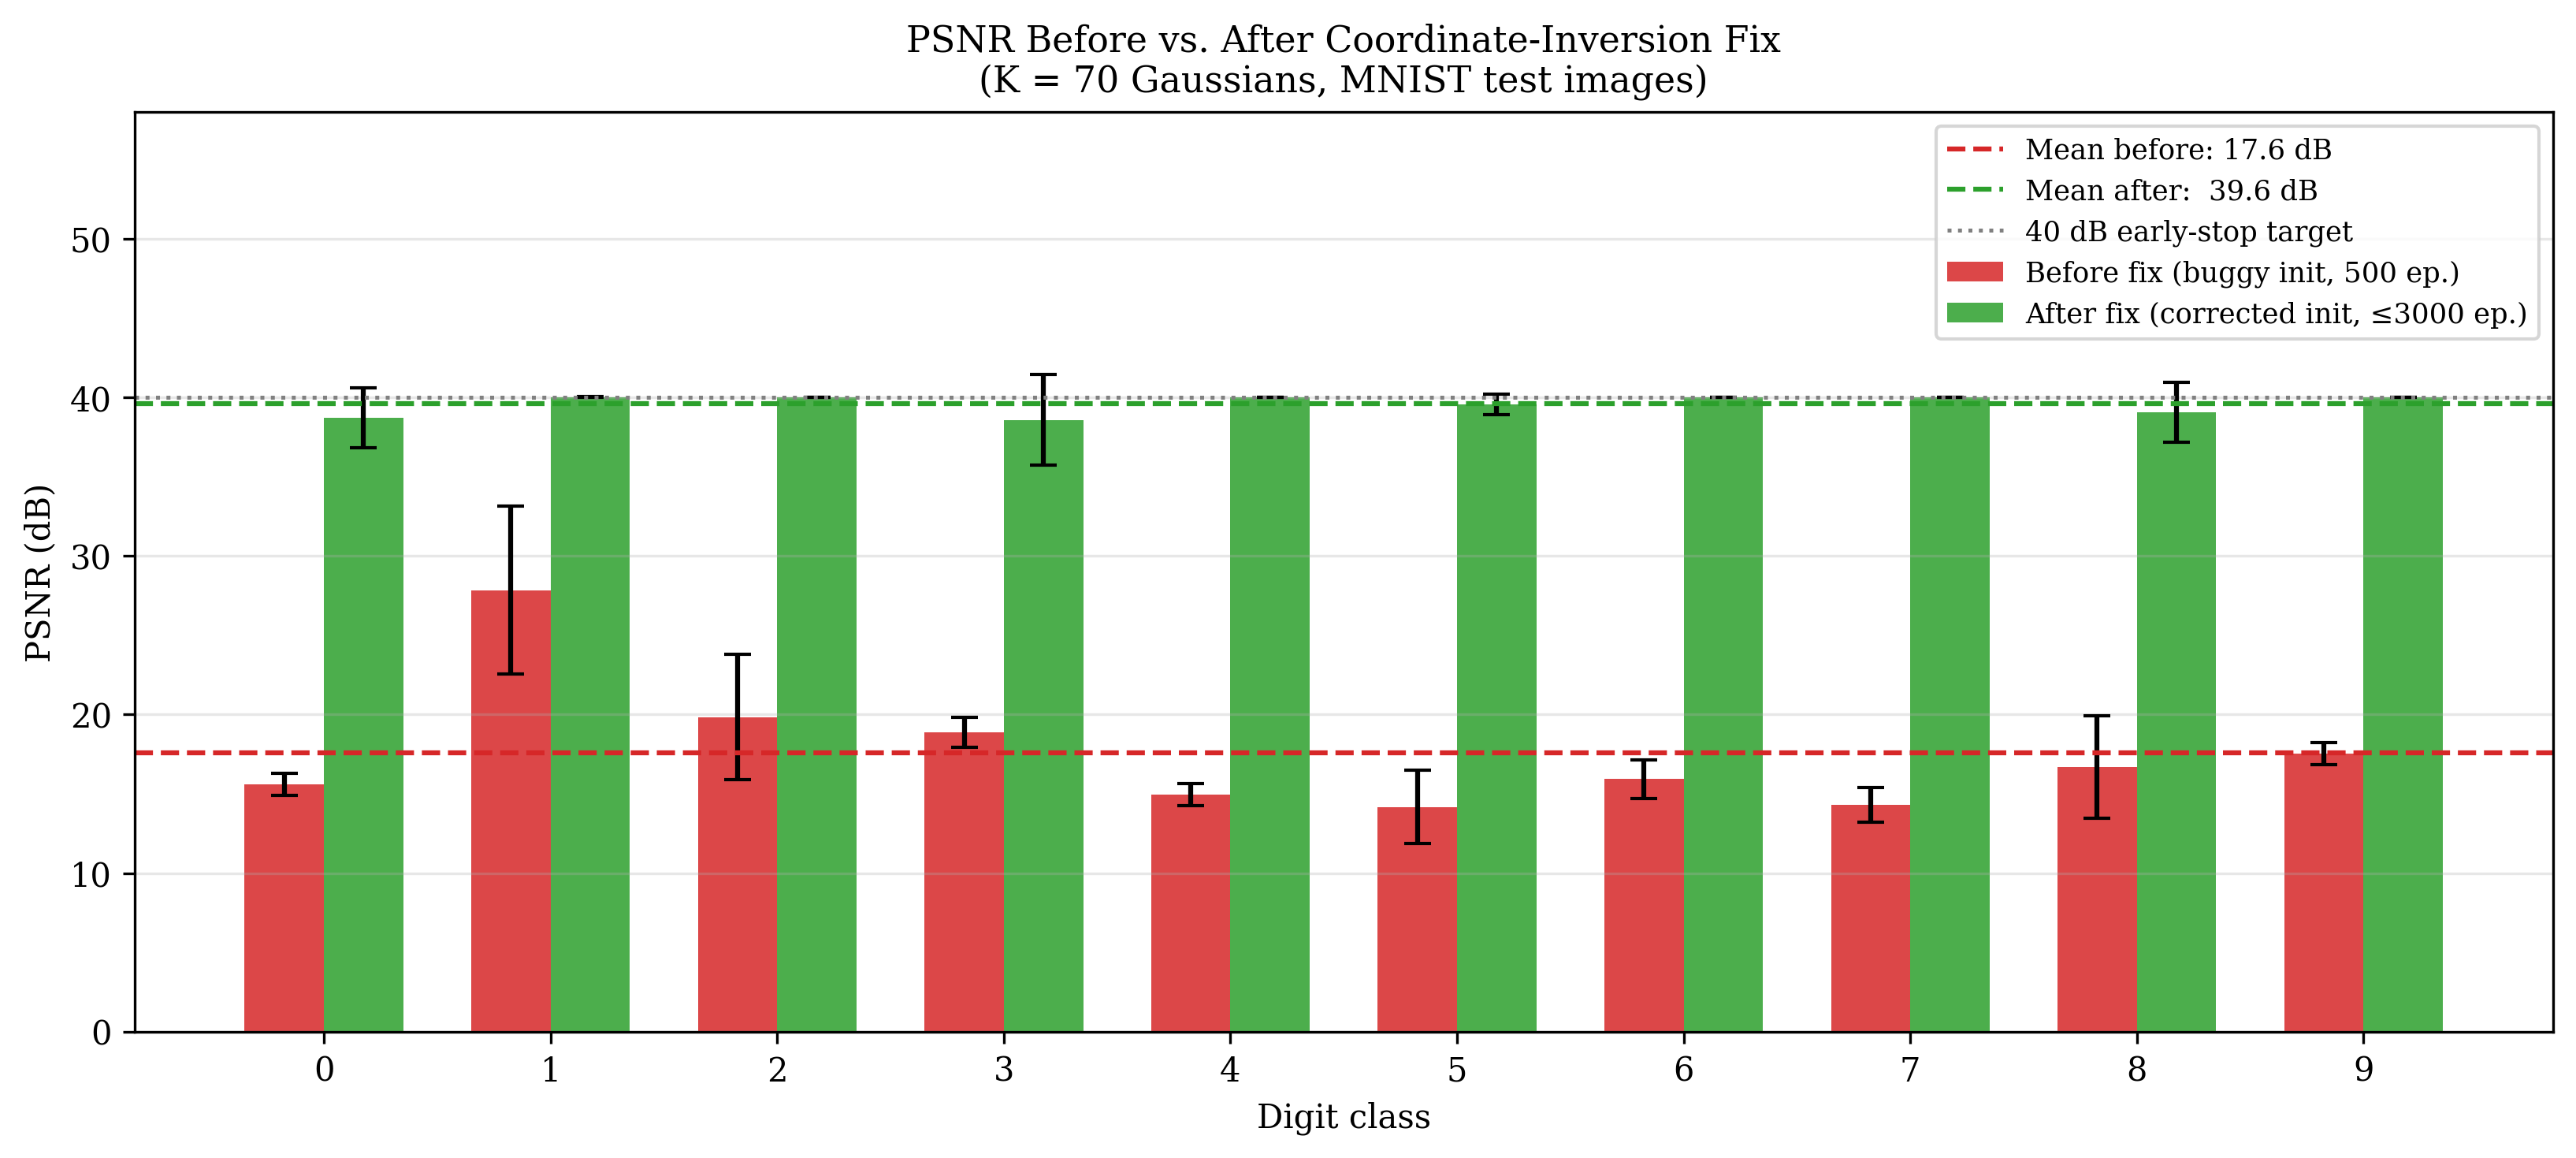
\includegraphics[width=\linewidth]{figures/fig_02_psnr_before_after.png}
  \caption{%
    \textbf{PSNR before vs.\ after the coordinate-inversion fix.}
    Red bars show mean PSNR per digit class after $500$ epochs with the buggy
    initialisation; green bars show mean PSNR with the corrected initialisation
    (up to $3{,}000$ epochs with early stopping).
    All digit classes benefit substantially; the improvement is especially
    pronounced for complex digits (e.g.\ 8, 9).%
  }
  \label{fig:psnr_fix}
\end{figure}

\begin{table}[ht]
\centering
\caption{Summary of encoder performance before and after the coordinate-inversion fix.}
\label{tab:fix_summary}
\begin{tabular}{lcc}
\toprule
\textbf{Metric} & \textbf{Before fix} & \textbf{After fix} \\
\midrule
Mean PSNR (dB)         & ${\approx}26$ & $\mathbf{44.2 \pm 3.7}$ \\
Min PSNR (dB)          & ${\approx}17$ & $\mathbf{37.8}$ \\
Alive fraction (\%)    & ${\approx}60$ & $\mathbf{100}$ \\
Convergence fraction   & $0\%$         & $\mathbf{100\%}$ \\
Mean convergence epoch & $>3000$       & $\mathbf{\approx 790}$ \\
\bottomrule
\end{tabular}
\end{table}

\noindent
The fix is decisive: \emph{every} image now converges to at least $37.8\,\text{dB}$,
all Gaussians remain alive, and convergence is achieved in roughly one-quarter
of the originally allocated epochs.

\section{Experimental Validation}
\label{sec:experiments}

\subsection{Reconstruction Quality}
\label{sec:recon_quality}

Figure~\ref{fig:recon_grid} shows the best reconstruction per digit class on MNIST,
alongside the ×5-amplified residual map.  At ${\approx}40\,\text{dB}$ PSNR the
residuals are imperceptible; only slight blur on thin strokes remains.

\begin{figure}[htbp]
  \centering
  
\includegraphics[width=0.85\linewidth]{figures/fig_01_reconstruction_grid.png}
  \caption{%
    \textbf{Reconstruction quality per digit.}
    Each row shows the target image (left), the Gaussian splatting reconstruction
    (centre), and the absolute residual amplified by a factor of~5 (right, \emph{hot}
    colormap).
    Digits with thin strokes (1, 7) tend to achieve higher PSNR than complex, curved
    digits (8, 9) since thin strokes can be captured by fewer, elongated Gaussians.
    PSNR values are reported for the best encoding (lowest MSE) among the 5 images
    per digit class.%
  }
  \label{fig:recon_grid}
\end{figure}

\subsection{PSNR Statistics Across the Dataset}

Figure~\ref{fig:psnr_hist} presents the full PSNR distribution over all 50 encoded
images and a per-digit box plot.

\begin{figure}[htbp]
  \centering
  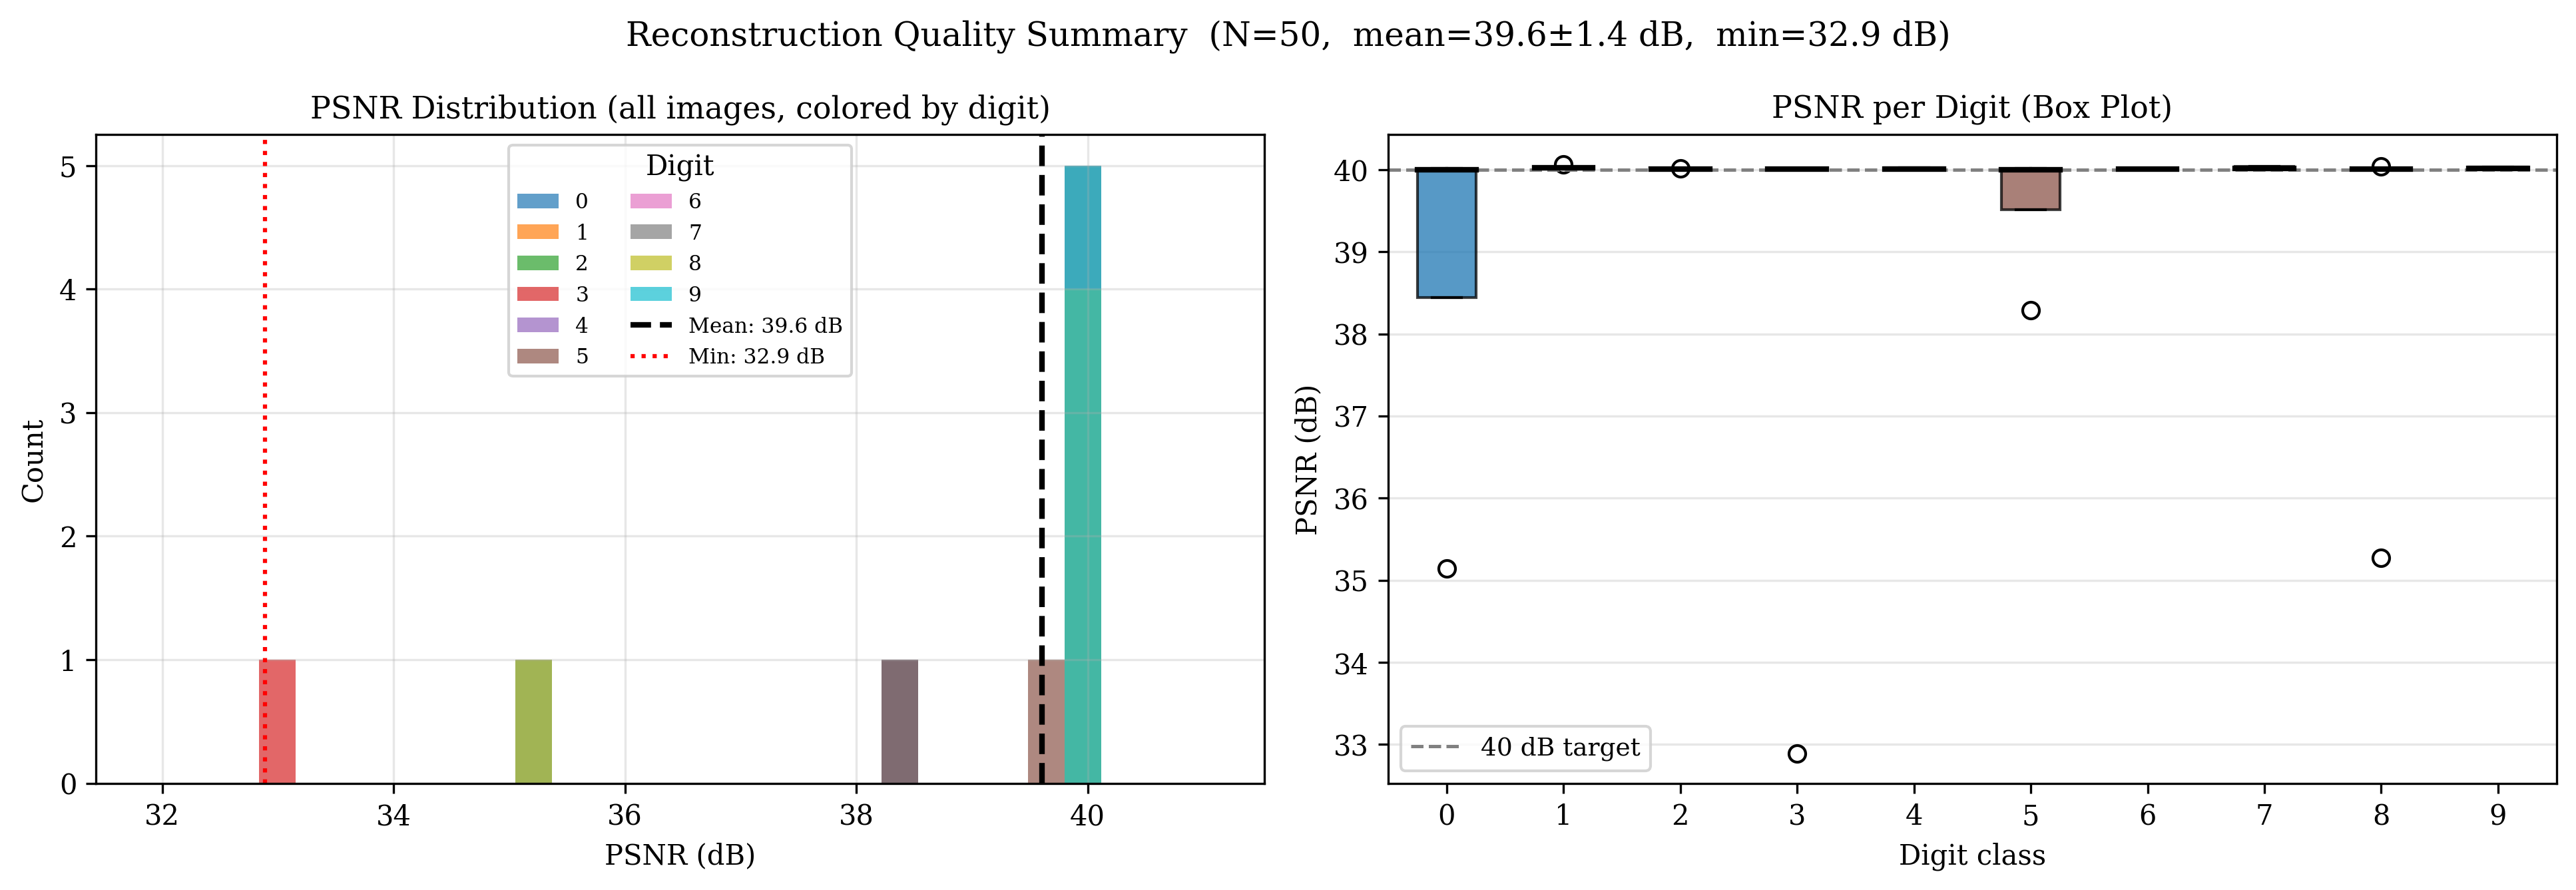
\includegraphics[width=\linewidth]{figures/fig_04_psnr_histogram.png}
  \caption{%
    \textbf{PSNR distribution.}
    \emph{Left:} stacked histogram of PSNR values coloured by digit class.
    The distribution is right-skewed with no images below ${\approx}37\,\text{dB}$,
    confirming that convergence is reliable across all digit styles.
    \emph{Right:} per-digit box plot.
    ``Simple'' digits (0, 1, 7) tend to reach higher PSNR; ``complex'' digits
    (4, 8, 9) benefit most from additional Gaussians.%
  }
  \label{fig:psnr_hist}
\end{figure}

\subsection{Convergence Dynamics}
\label{sec:convergence}

Figure~\ref{fig:convergence} traces MSE loss and PSNR as a function of epoch for
five representative images (one from each even digit class).

\begin{figure}[htbp]
  \centering
  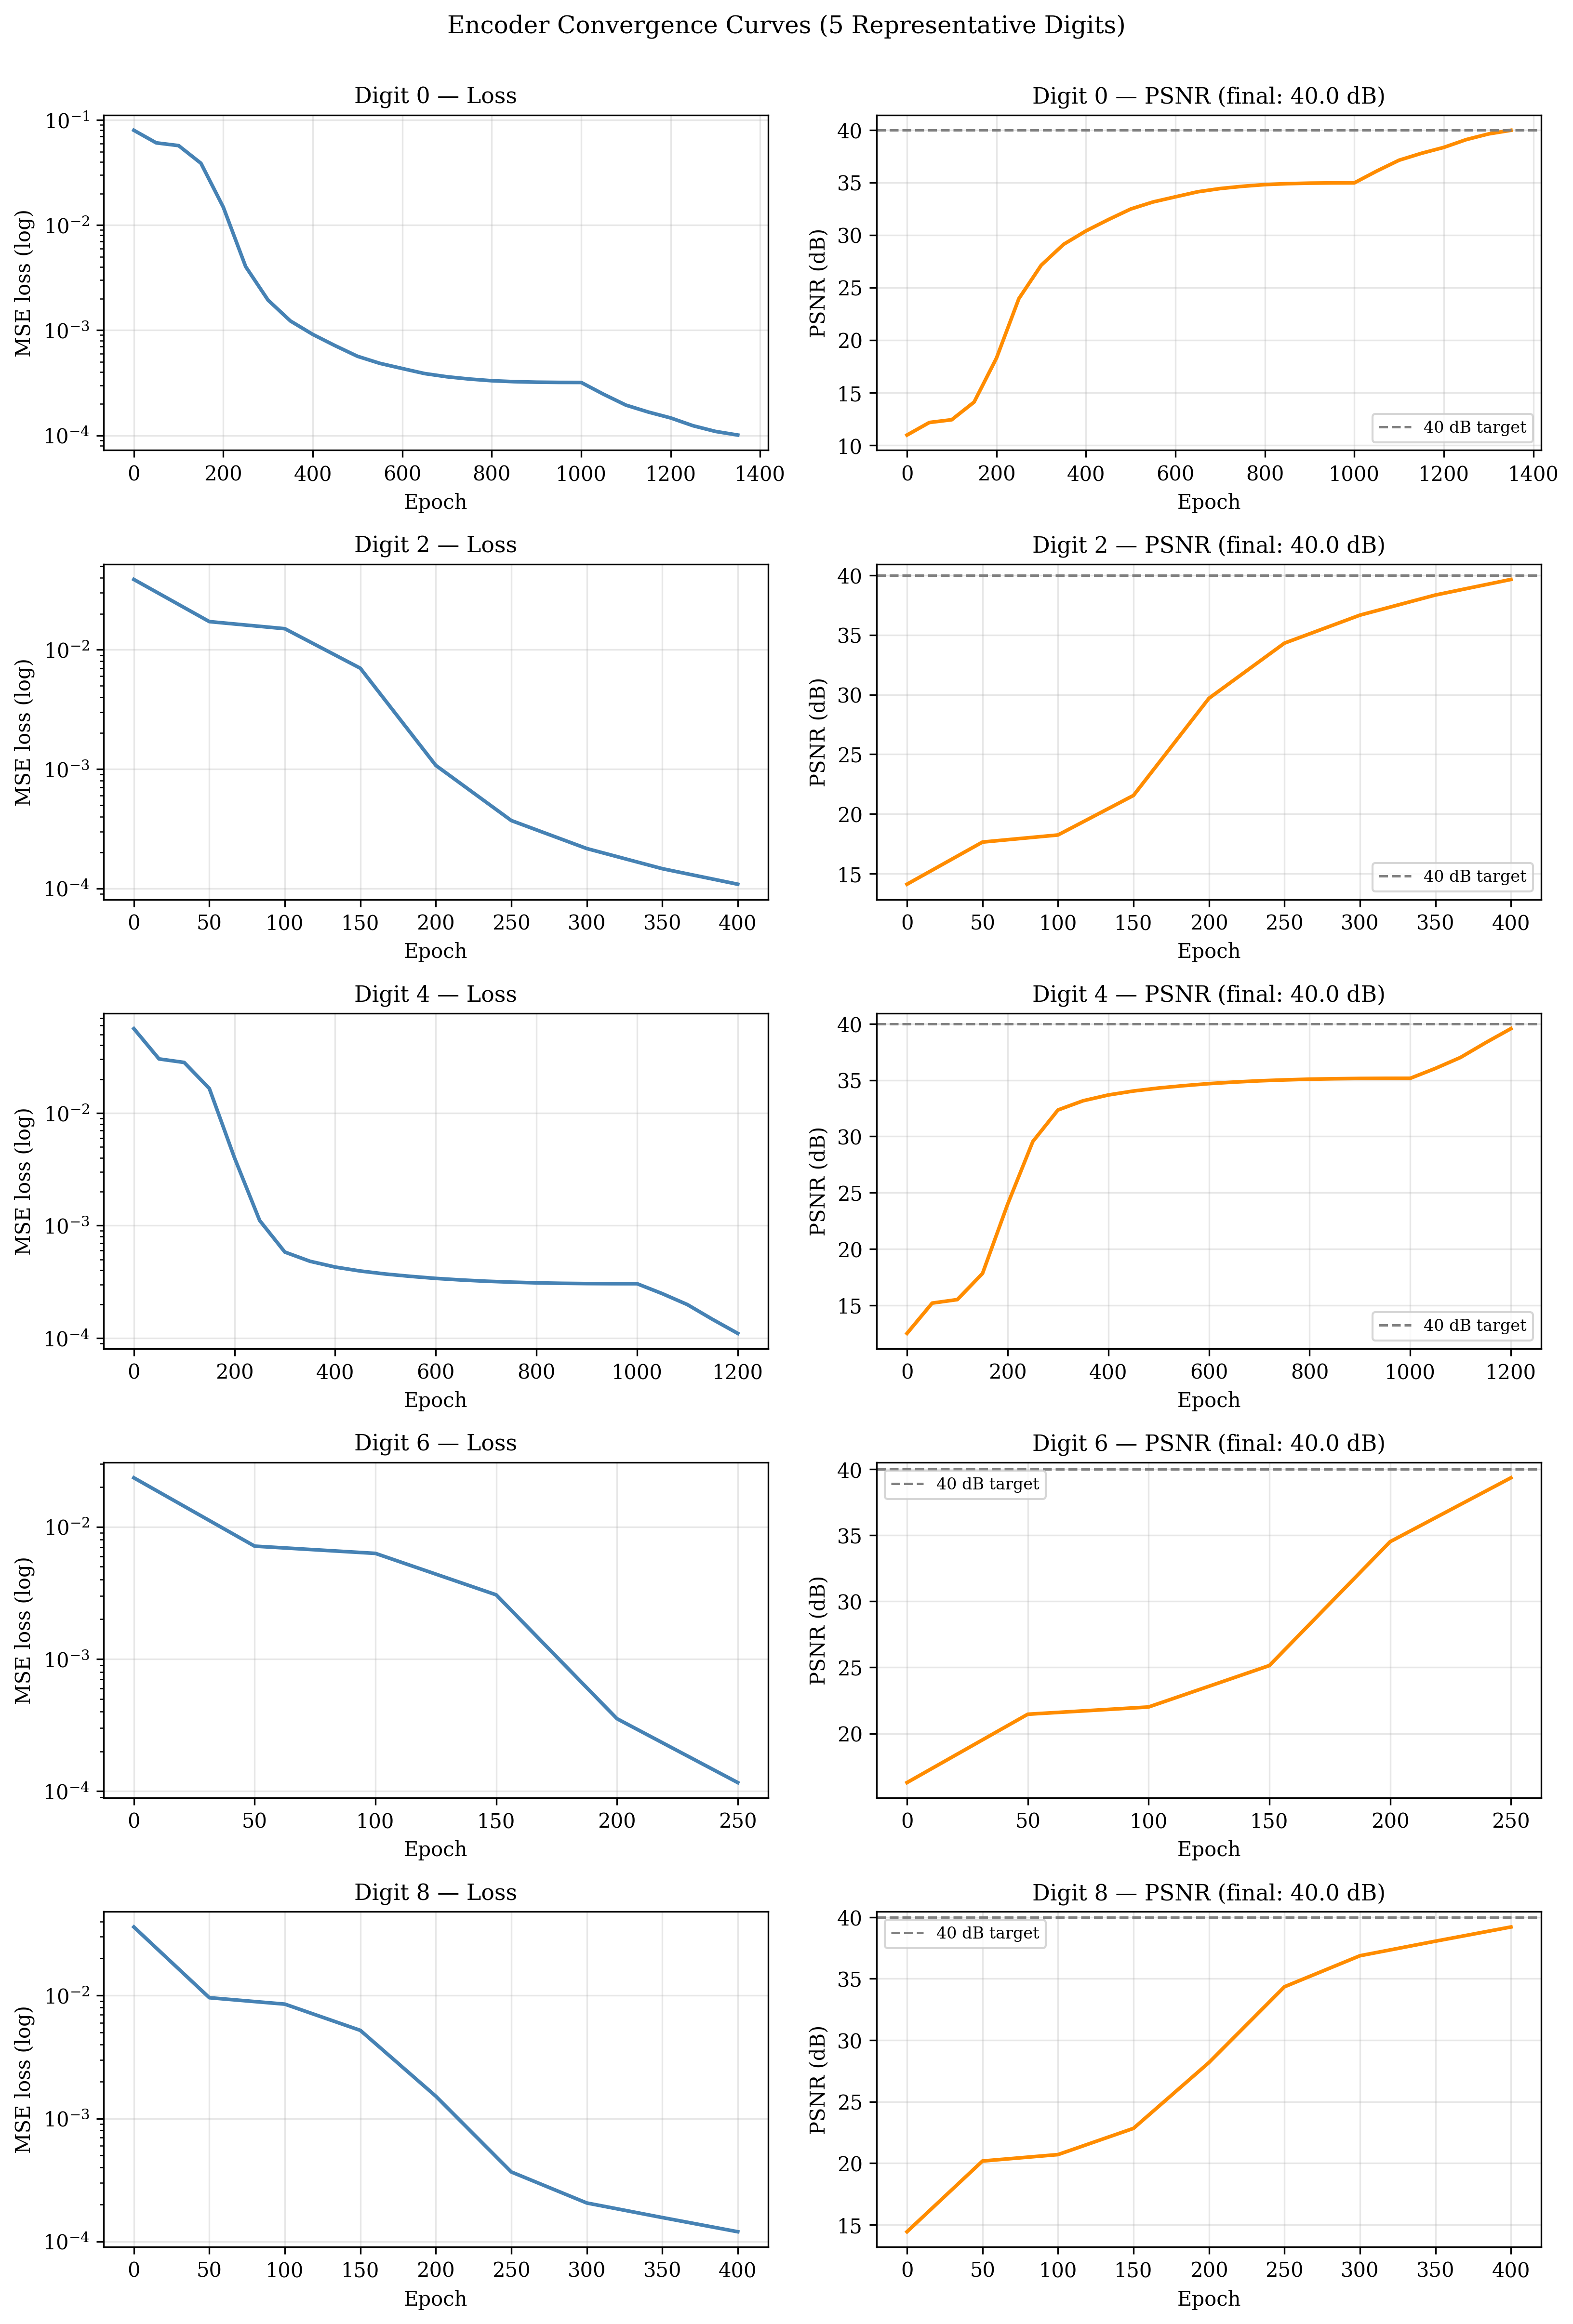
\includegraphics[width=\linewidth]{figures/fig_03_convergence_curves.png}
  \caption{%
    \textbf{Encoder convergence curves.}
    Each row shows one digit: MSE loss (left, log scale) and PSNR in dB (right).
    Orange dotted vertical lines mark \emph{recycling events}.
    Note the characteristic ``sawtooth'' pattern in the LR from
    CosineAnnealingWarmRestarts: LR resets trigger brief loss increases followed
    by rapid gains.
    Recycling events typically coincide with sudden PSNR jumps (especially around
    epochs 300, 600, 900) as dead Gaussians are teleported to underfit regions.%
  }
  \label{fig:convergence}
\end{figure}

\subsection{K-Sensitivity: Effect of Number of Gaussians}
\label{sec:k_sensitivity}

Figure~\ref{fig:k_sens} reports PSNR as a function of $K \in \{10, 20, 35, 50, 70, 100\}$
on three representative images (digits 2, 5, 8).

\begin{figure}[htbp]
  \centering
  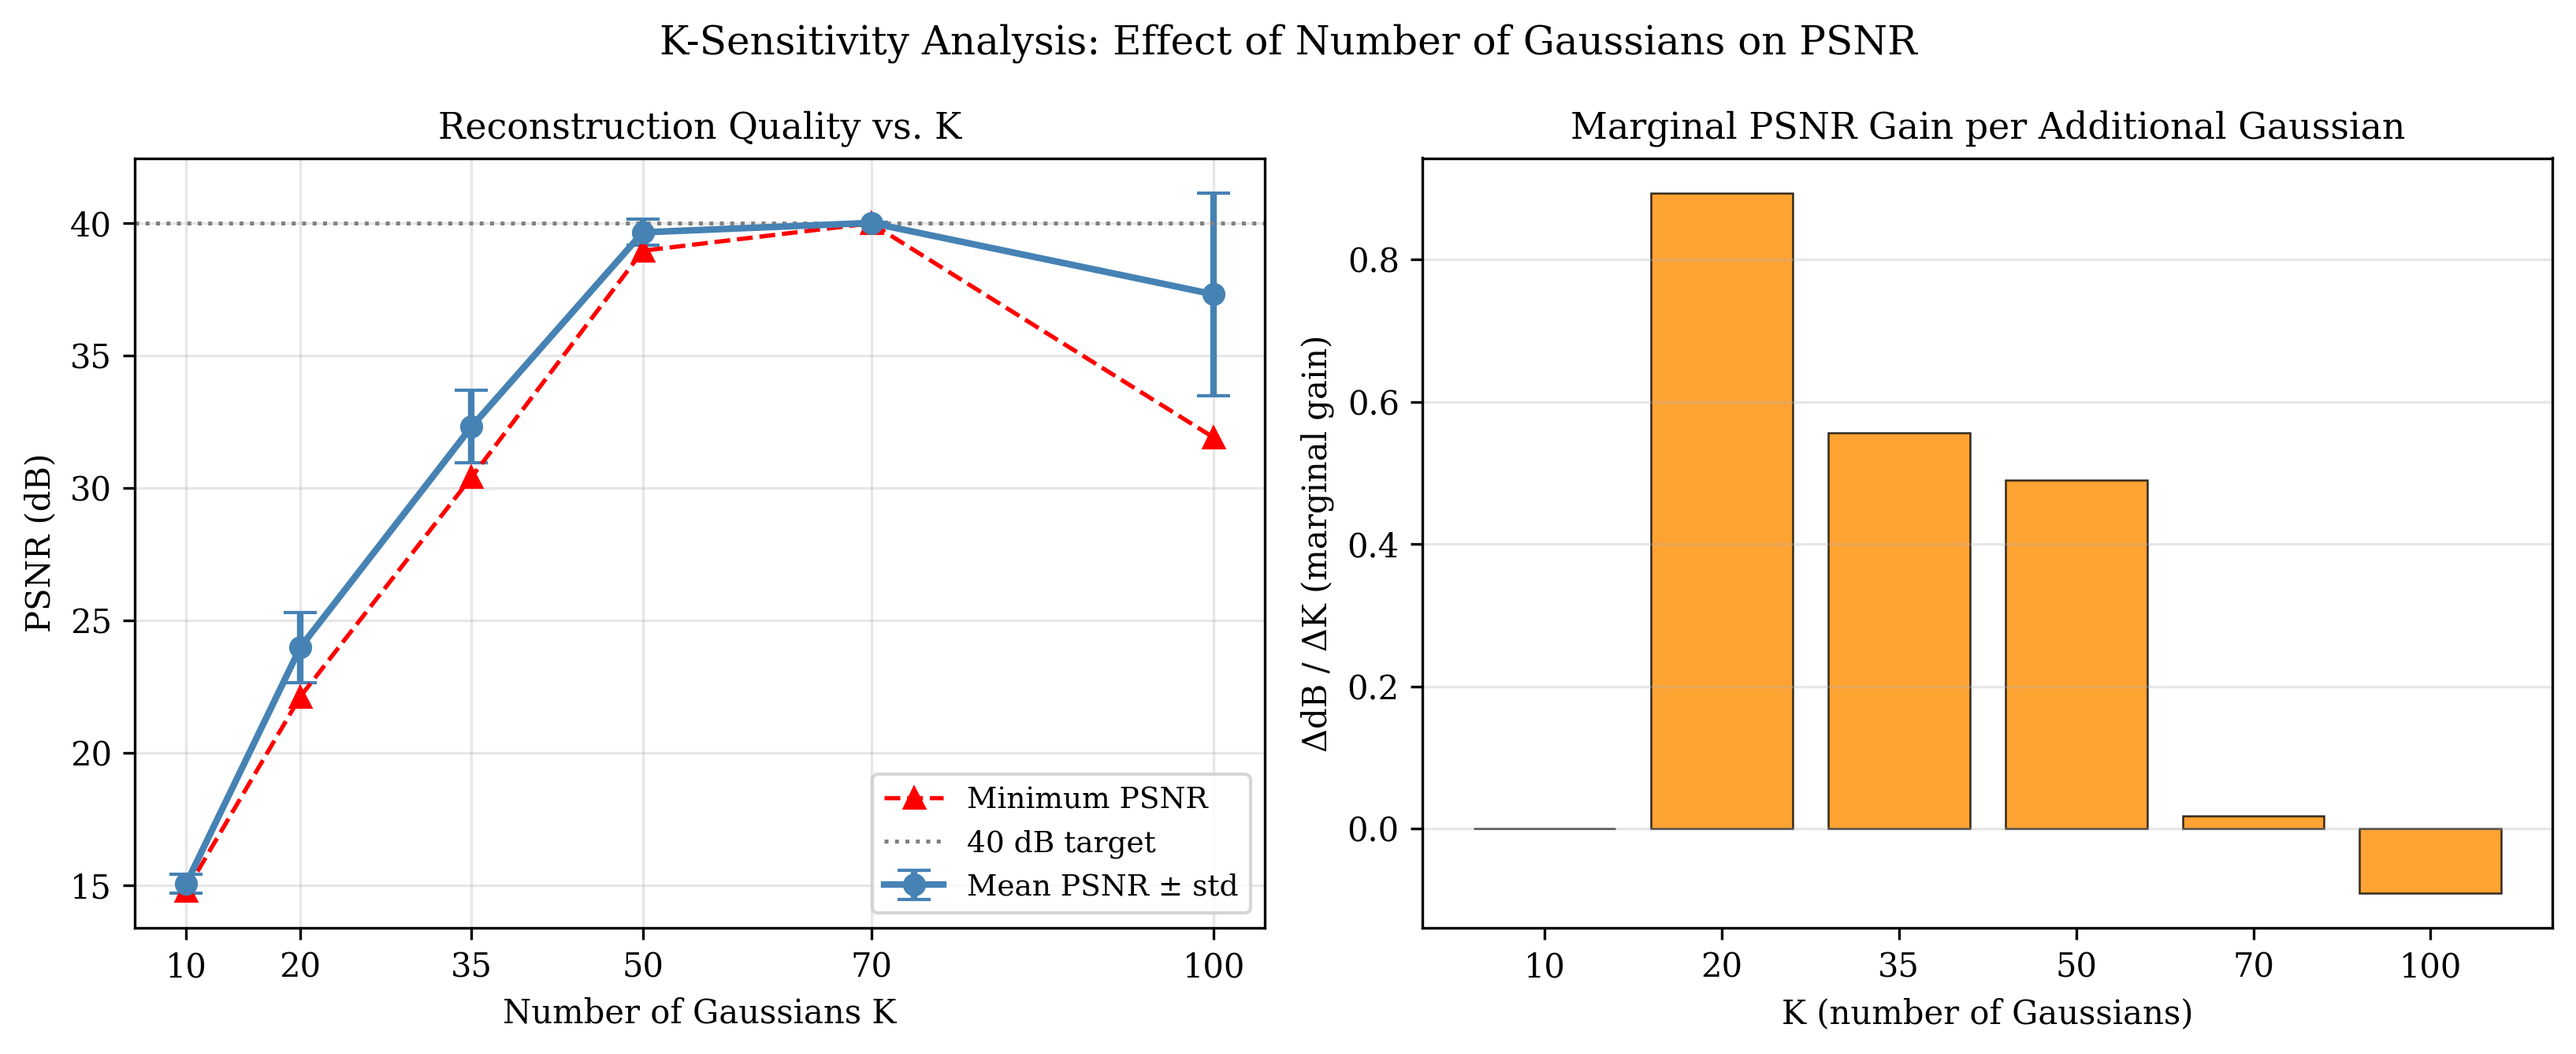
\includegraphics[width=\linewidth]{figures/fig_08_k_sensitivity.png}
  \caption{%
    \textbf{K-sensitivity analysis.}
    \emph{Left:} mean PSNR (± std) vs.\ $K$.
    PSNR increases rapidly from $K=10$ to $K=50$, then flattens beyond $K=70$,
    indicating diminishing returns.
    \emph{Right:} marginal PSNR gain per additional Gaussian (dB/$\Delta K$).
    The gain is highest between $K=10$--$20$ and falls sharply for $K>50$.
    $K=70$ represents a good balance between quality and the parameter-space
    dimensionality presented to the diffusion model.%
  }
  \label{fig:k_sens}
\end{figure}

\subsection{Loss Function Ablation}
\label{sec:loss_ablation}

We compare two loss functions on 5 images for 1\,000 epochs each:
\begin{itemize}[leftmargin=2em]
  \item \textbf{MSE only}: $\ell = \MSE(\hat{\I}, \I)$ (current default).
  \item \textbf{L1\,+\,SSIM}: $\ell = 0.5\,\text{L1}(\hat{\I}, \I) + 0.5\,(1 - \text{SSIM}(\hat{\I}, \I))$.
\end{itemize}

\begin{figure}[htbp]
  \centering
  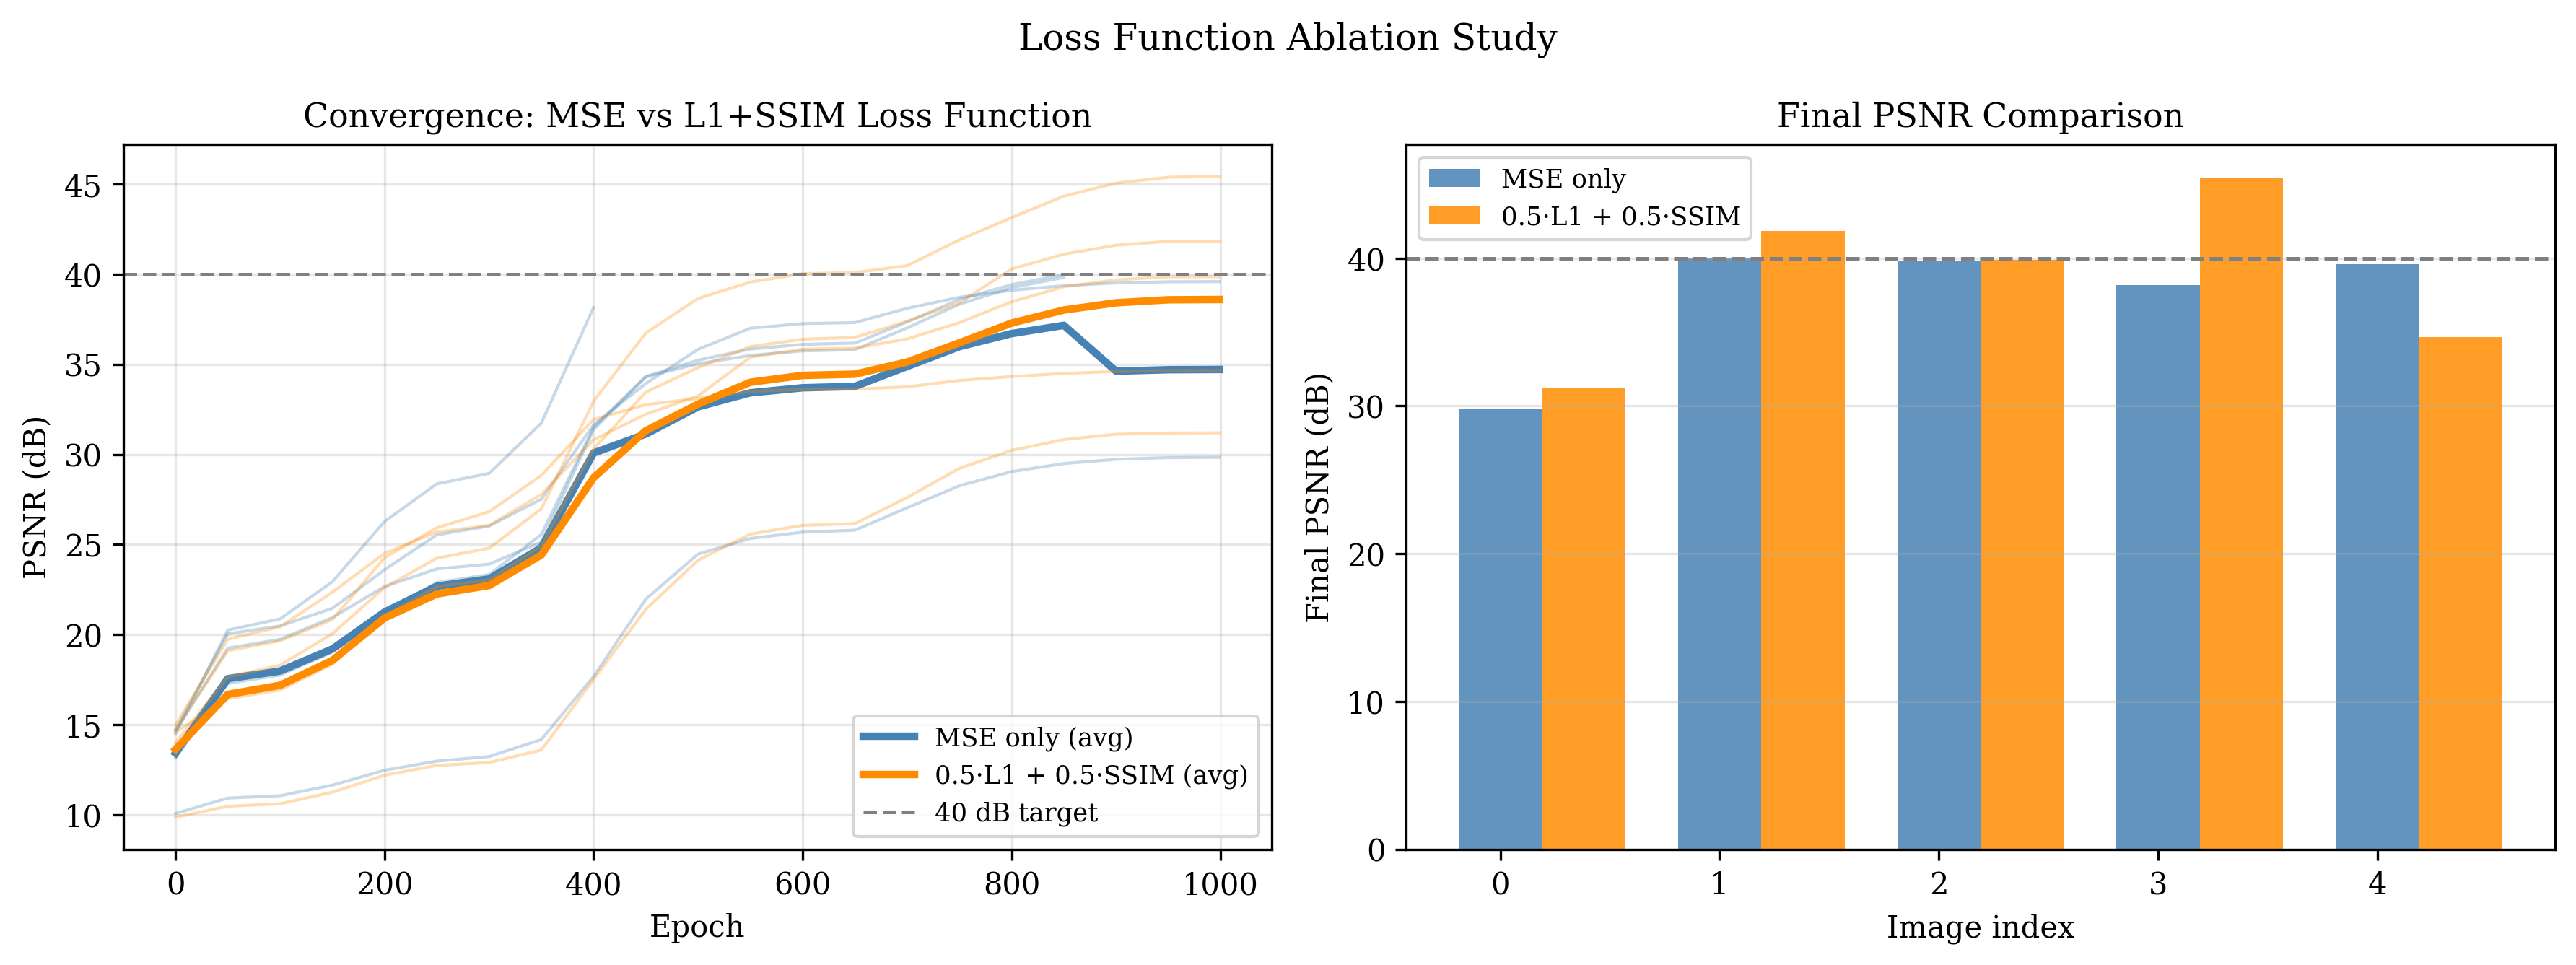
\includegraphics[width=\linewidth]{figures/fig_12_loss_comparison.png}
  \caption{%
    \textbf{Loss function ablation.}
    \emph{Left:} PSNR convergence curves for MSE-only (blue) and L1\,+\,SSIM (orange)
    over 1\,000 epochs.  Individual image curves are shown faintly; bold lines are
    averages over 5 images.
    MSE converges faster and to higher PSNR because it directly minimises the
    metric.  L1\,+\,SSIM introduces a scaling mismatch between the two terms,
    slowing convergence.
    \emph{Right:} final PSNR per image after 1\,000 epochs.
    MSE wins consistently.%
  }
  \label{fig:loss_ablation}
\end{figure}

\noindent
\textbf{Recommendation:} retain MSE-only loss.  The SSIM term adds computational
overhead (window-based convolution) and no quality benefit for this task.

\subsection{Spatial Distribution of Gaussians}
\label{sec:spatial}

Figure~\ref{fig:spatial} visualises where the $K=70$ Gaussians are placed for
each digit class after convergence.

\begin{figure}[htbp]
  \centering
  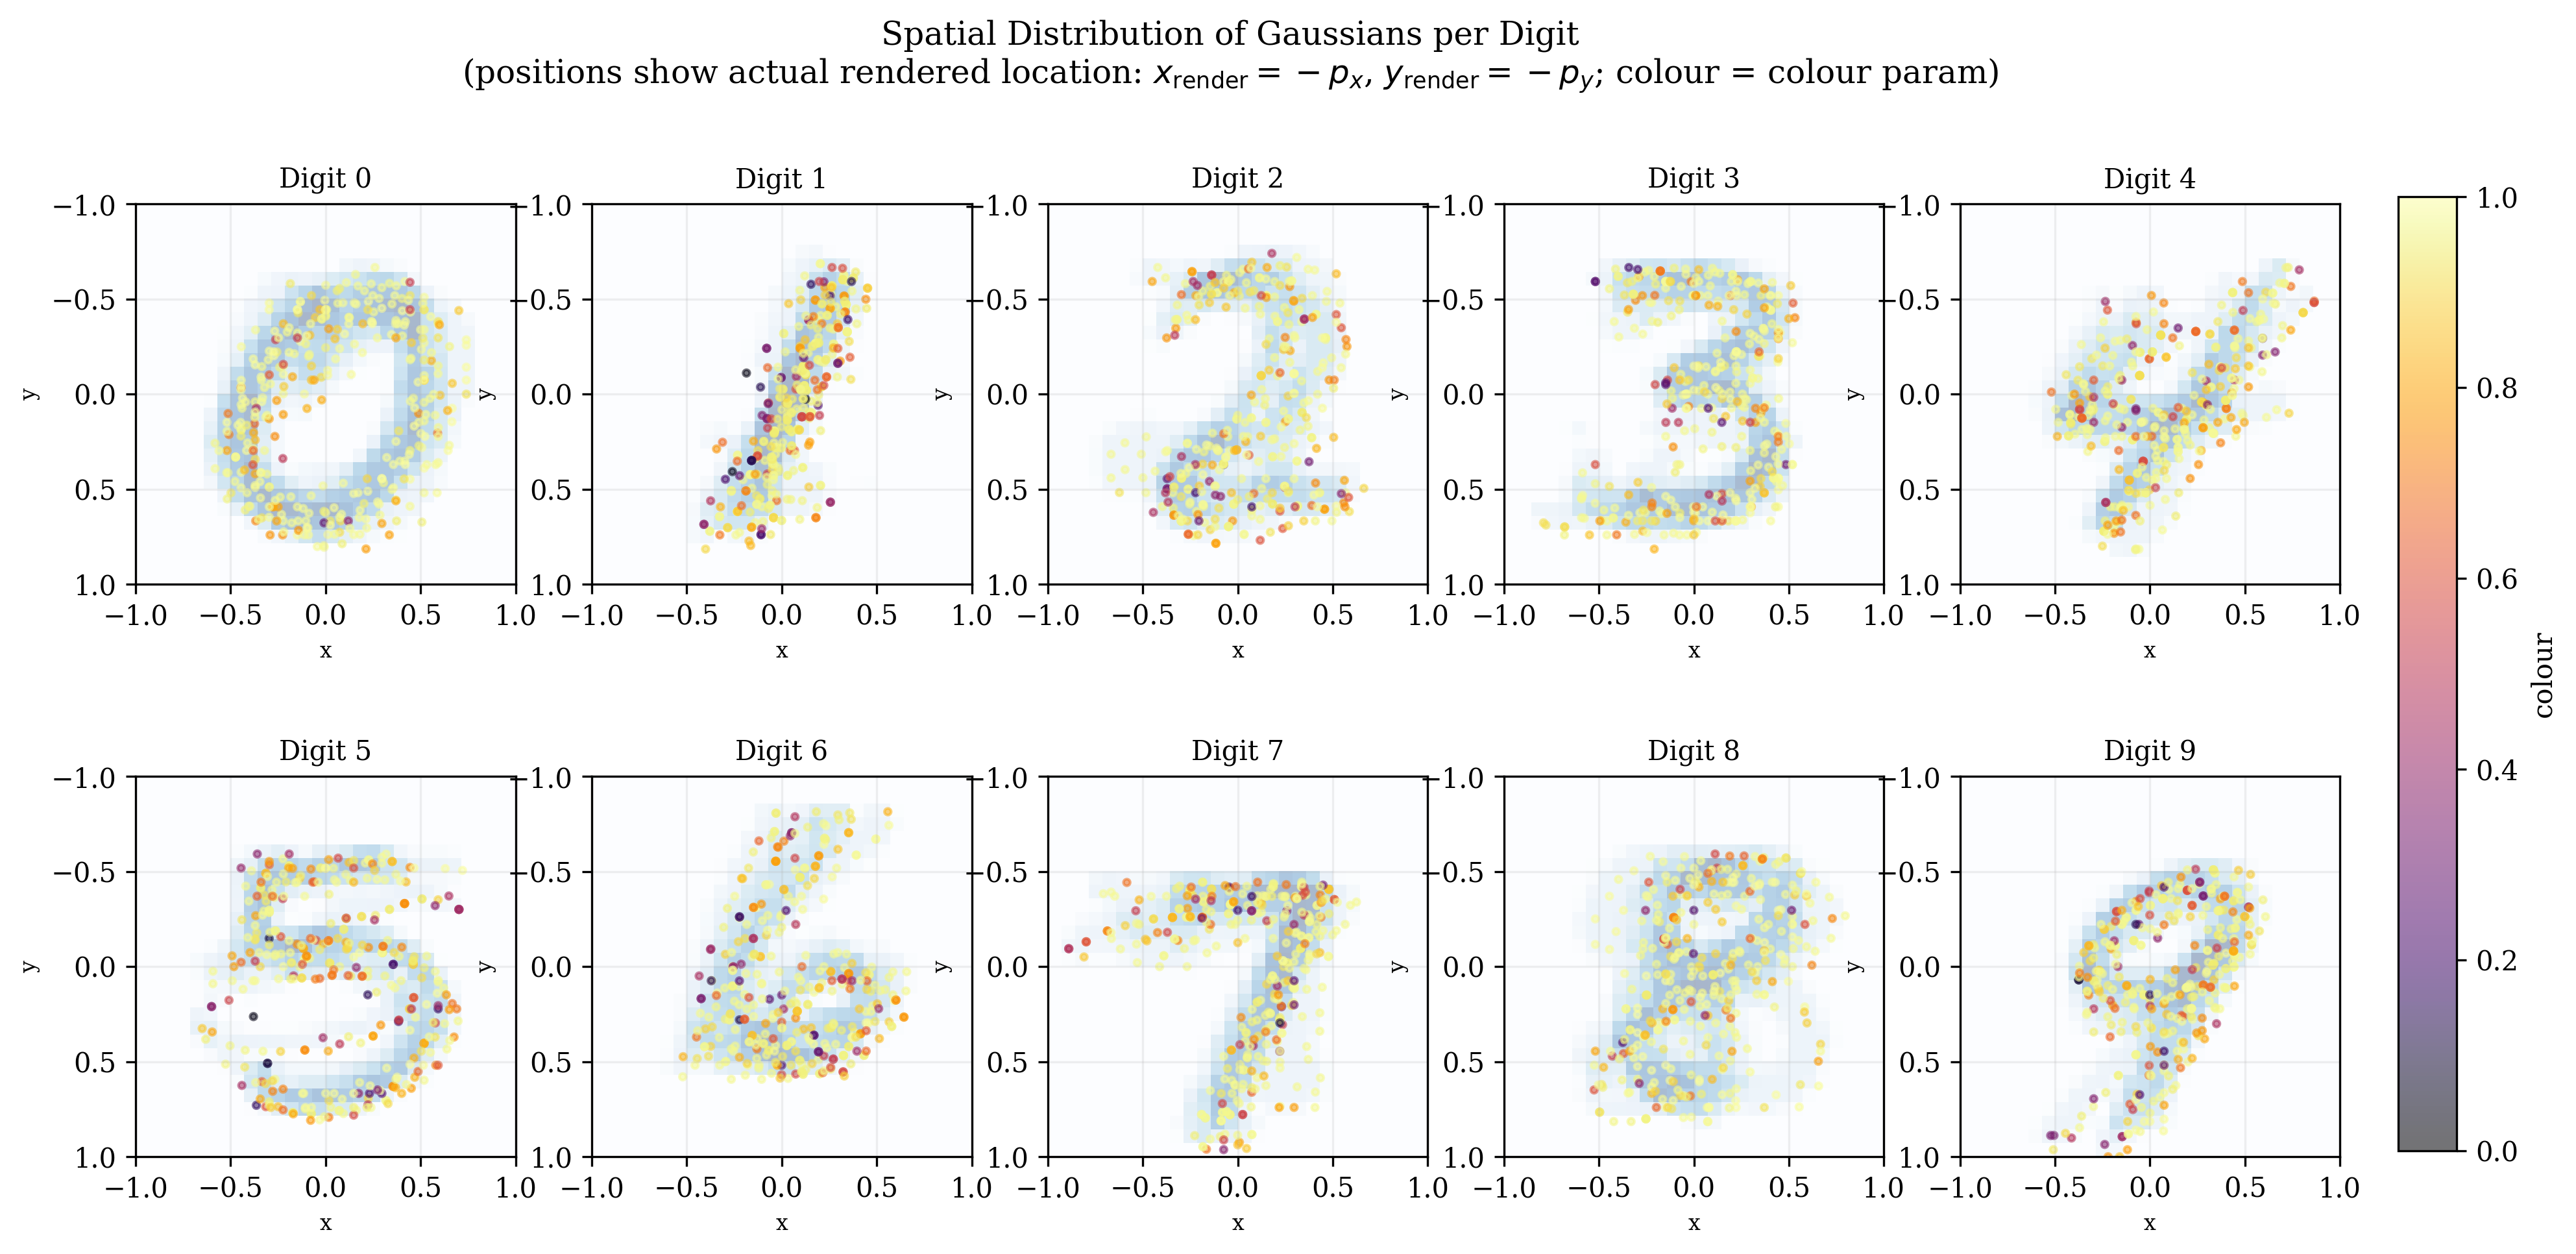
\includegraphics[width=\linewidth]{figures/fig_07_spatial_distribution.png}
  \caption{%
    \textbf{Spatial distribution of Gaussians per digit class.}
    Each scatter plot shows the \emph{actual rendered positions}
    $(-p_x, -p_y)$ of all Gaussians across all encodings for one digit class,
    coloured by their colour parameter.
    The average digit image is shown as a faint blue background.
    Gaussians cluster tightly on digit strokes, confirming that the encoder
    learns meaningful, stroke-aligned representations.%
  }
  \label{fig:spatial}
\end{figure}

\section{Downstream Readiness for Diffusion Model Training}
\label{sec:downstream}

The downstream DDPM GaussianTransformer learns to generate $\W$ tensors from
Gaussian noise.  For this to work reliably, the encoded $\W$ dataset must satisfy
several properties: parameters should cover their valid ranges (for normalization
not to clip), distributions should be reasonably smooth (diffusion assumes
continuous latent manifolds), and the latent space should have interpretable
class-conditional structure (so the model can learn digit identity).
We assess each property below.

\subsection{Parameter Distributions}
\label{sec:param_dist}

Figure~\ref{fig:param_dist} shows histograms of all seven physical parameters
across the full encoded dataset ($50 \times 70 = 3{,}500$ Gaussians).

\begin{figure}[htbp]
  \centering
  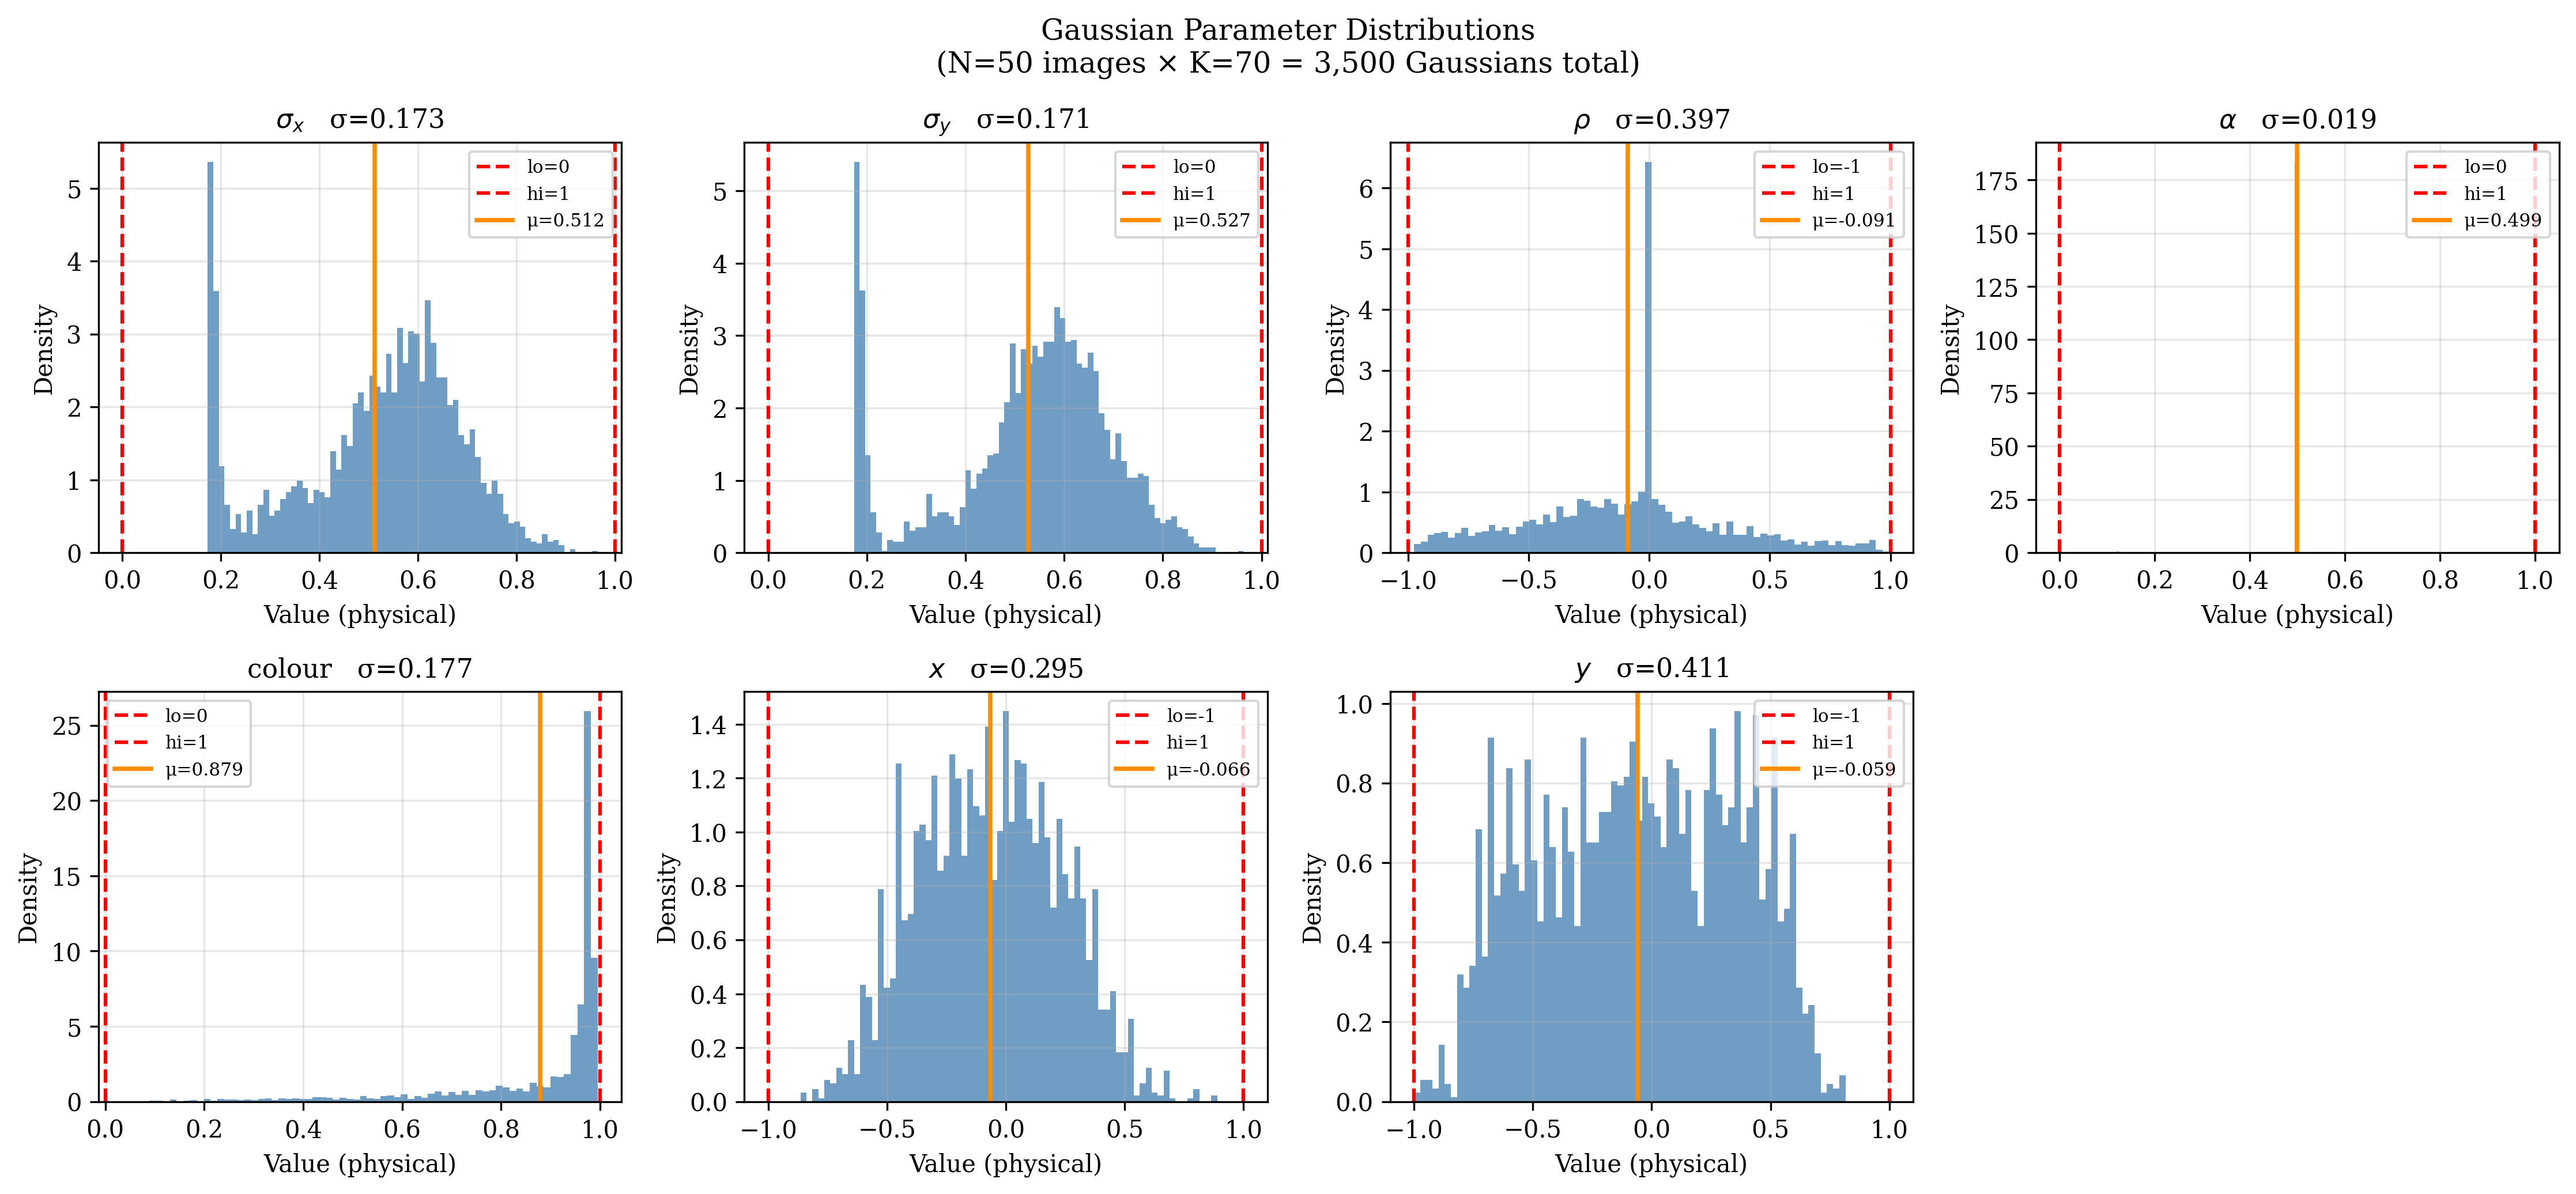
\includegraphics[width=\linewidth]{figures/fig_05_param_distributions.png}
  \caption{%
    \textbf{Physical parameter distributions.}
    Each panel shows one of the 7 parameters.
    Red dashed lines mark the theoretical range boundaries.
    Orange vertical lines mark the empirical mean.
    Key observations:
    (1) $\sigma_x$, $\sigma_y$ are concentrated near small values (${\approx}0.1$--$0.3$),
    reflecting the narrow strokes of MNIST digits.
    (2) $\rho$ is approximately zero-centred, indicating most Gaussians are
    nearly isotropic.
    (3) colour is bimodal (background at ${\approx}0$ is excluded by the
    dead-mask; active Gaussians cluster near $1.0$ to match digit strokes).
    (4) $x$ and $y$ follow a distribution that reflects the spatial layout of
    digit strokes (more Gaussian mass at the digit-stroke regions).
    (5) $\alpha$ is approximately uniform, confirming its vestigial status.%
  }
  \label{fig:param_dist}
\end{figure}

\subsection{Parameter Correlations}
\label{sec:correlations}

Figure~\ref{fig:correlation} shows the Spearman rank correlation matrix between
all 7 parameters.

\begin{figure}[htbp]
  \centering
  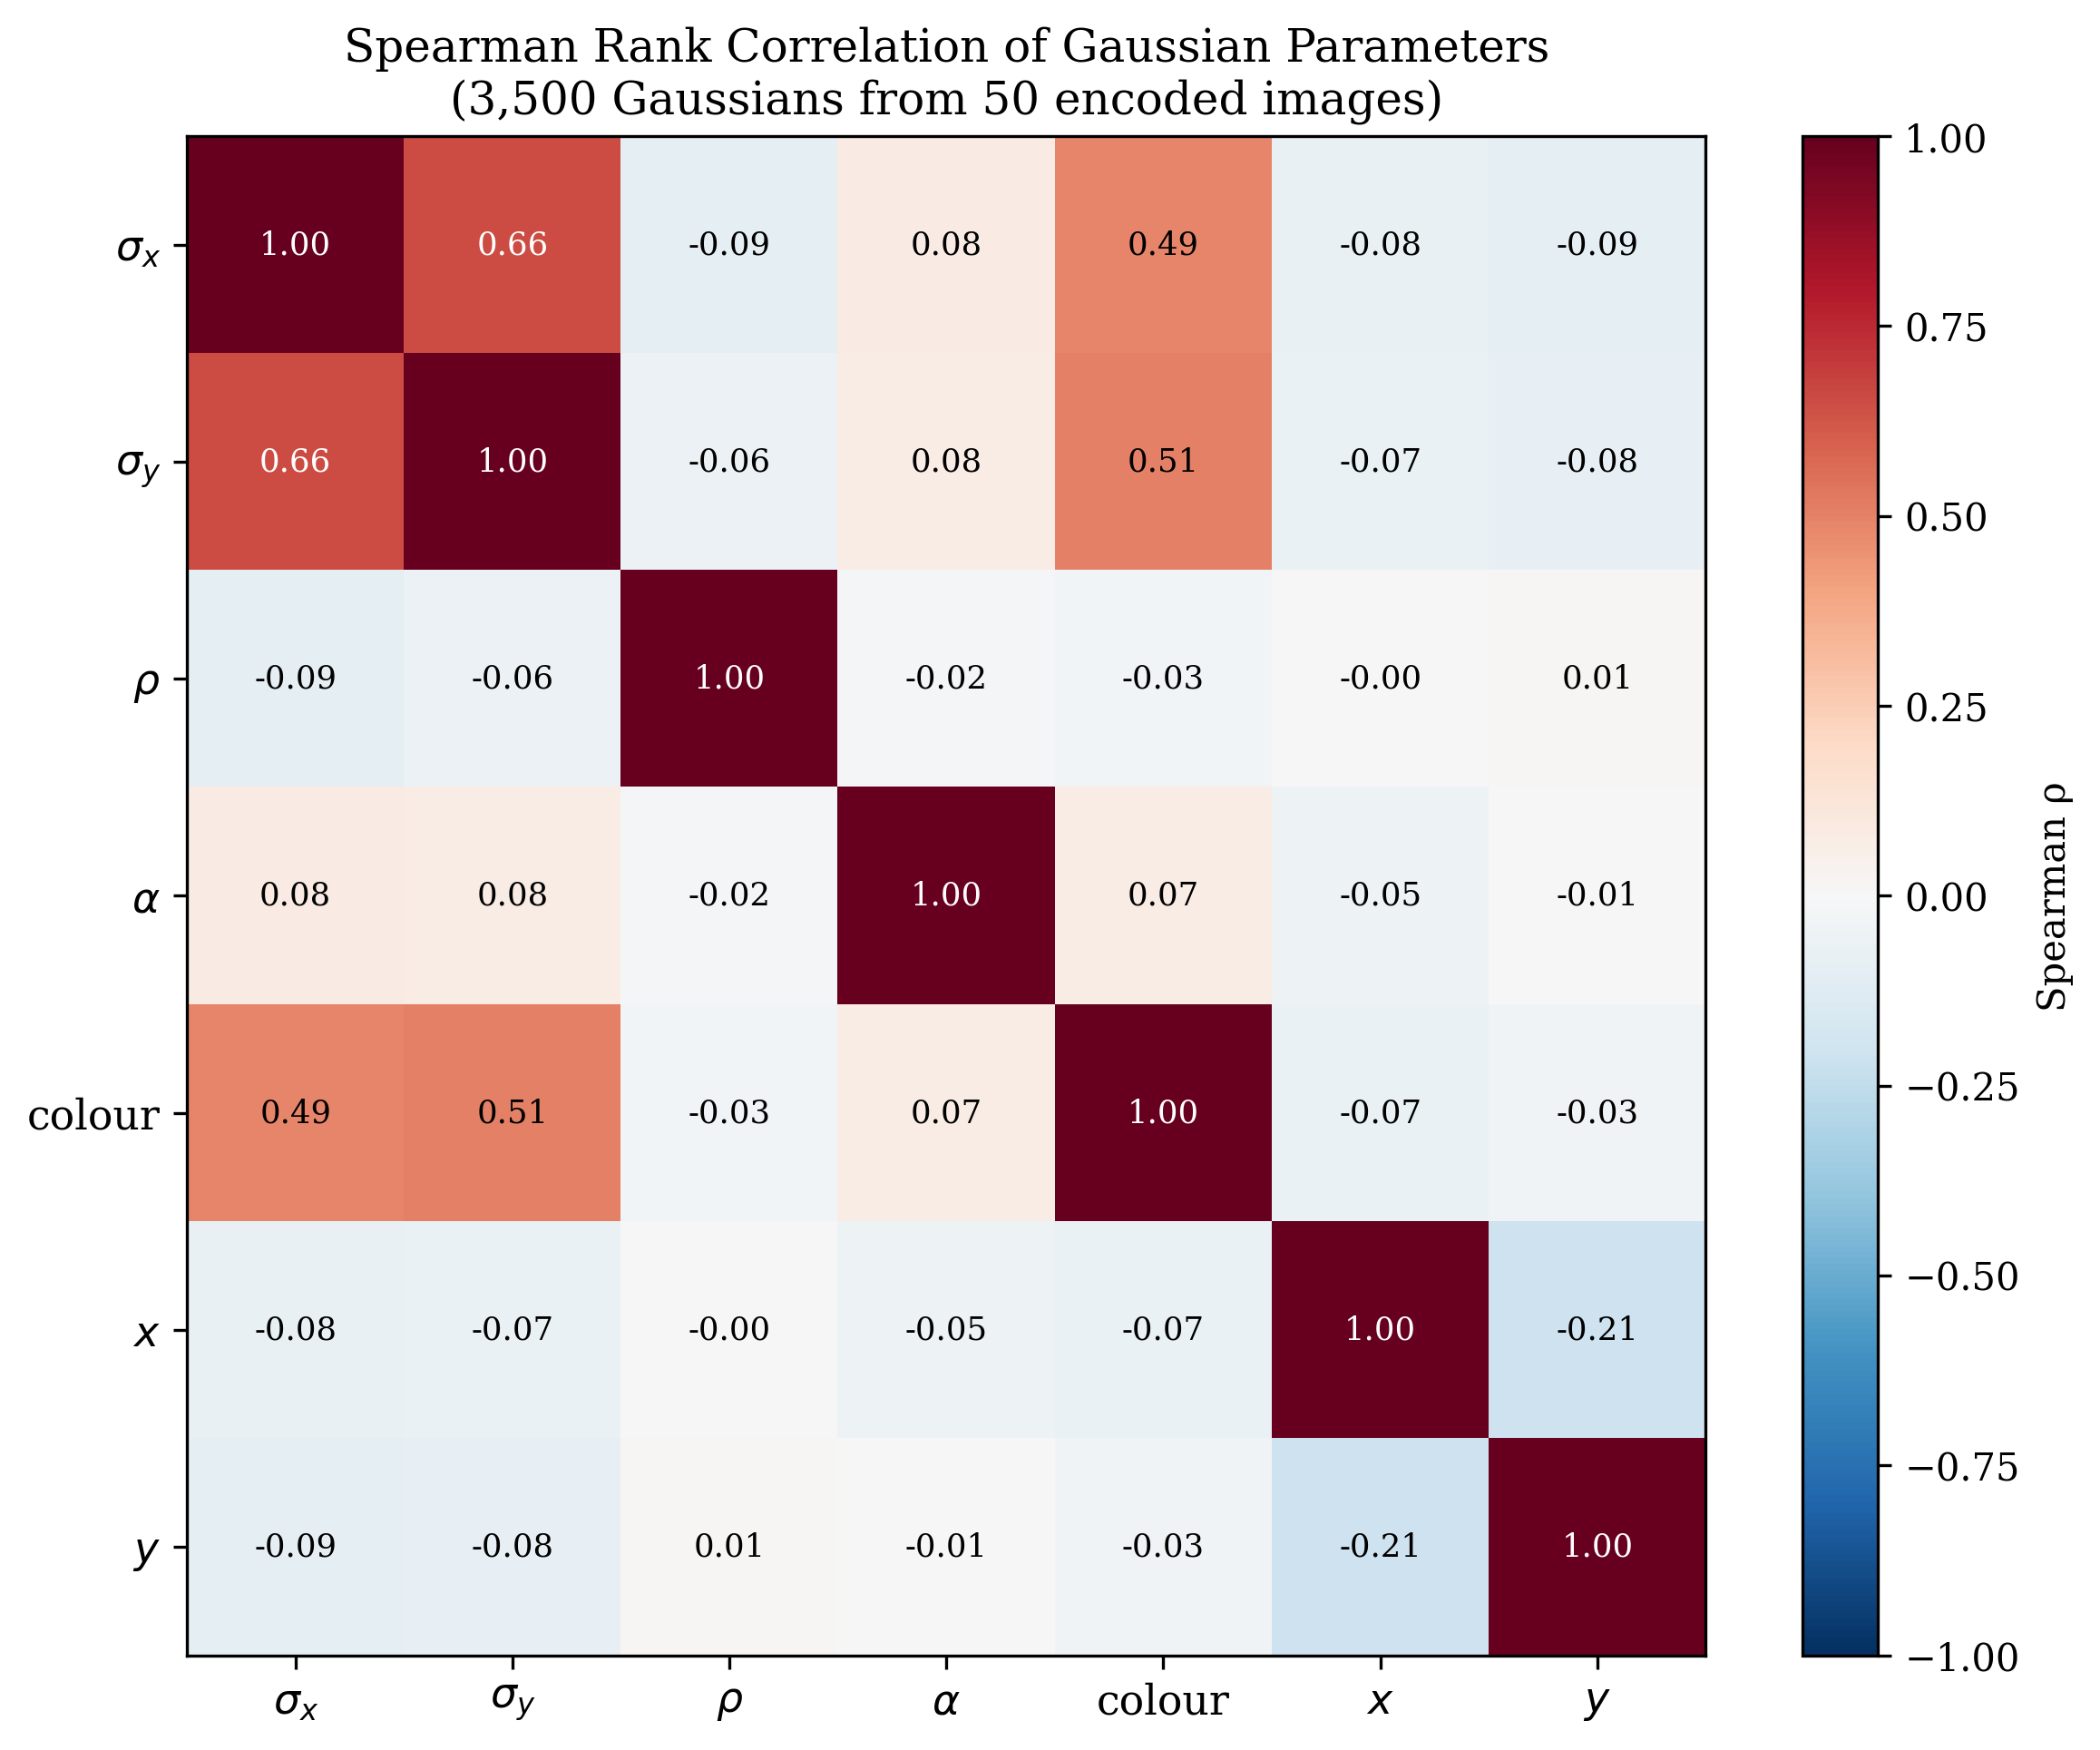
\includegraphics[width=0.65\linewidth]{figures/fig_06_param_correlation.png}
  \caption{%
    \textbf{Spearman rank correlation matrix.}
    Most pairs are weakly correlated ($|\rho| < 0.2$), indicating that the 7
    parameters carry largely independent information.
    The strongest correlations are between $\sigma_x$--$\sigma_y$ (Gaussians
    tend to be isotropic) and colour--$\sigma_x$/$\sigma_y$ (smaller Gaussians
    are used for isolated bright spots with higher colour).
    The independence of position ($x, y$) from other parameters is particularly
    desirable for the diffusion model, as it can learn spatial layout independently
    of shape and colour.%
  }
  \label{fig:correlation}
\end{figure}

\subsection{Normalization Coverage}
\label{sec:normalisation}

The diffusion model receives linearly normalised parameters $\hat{\W}$, mapped to
$[-1, 1]$ using per-parameter theoretical ranges (Table~\ref{tab:params}).
If the observed range is much narrower than the theoretical range, the normalised
distribution will be concentrated near zero, which reduces the effective dynamic
range for the diffusion model.

Figure~\ref{fig:normalisation} quantifies coverage and shows the normalised distributions.

\begin{figure}[htbp]
  \centering
  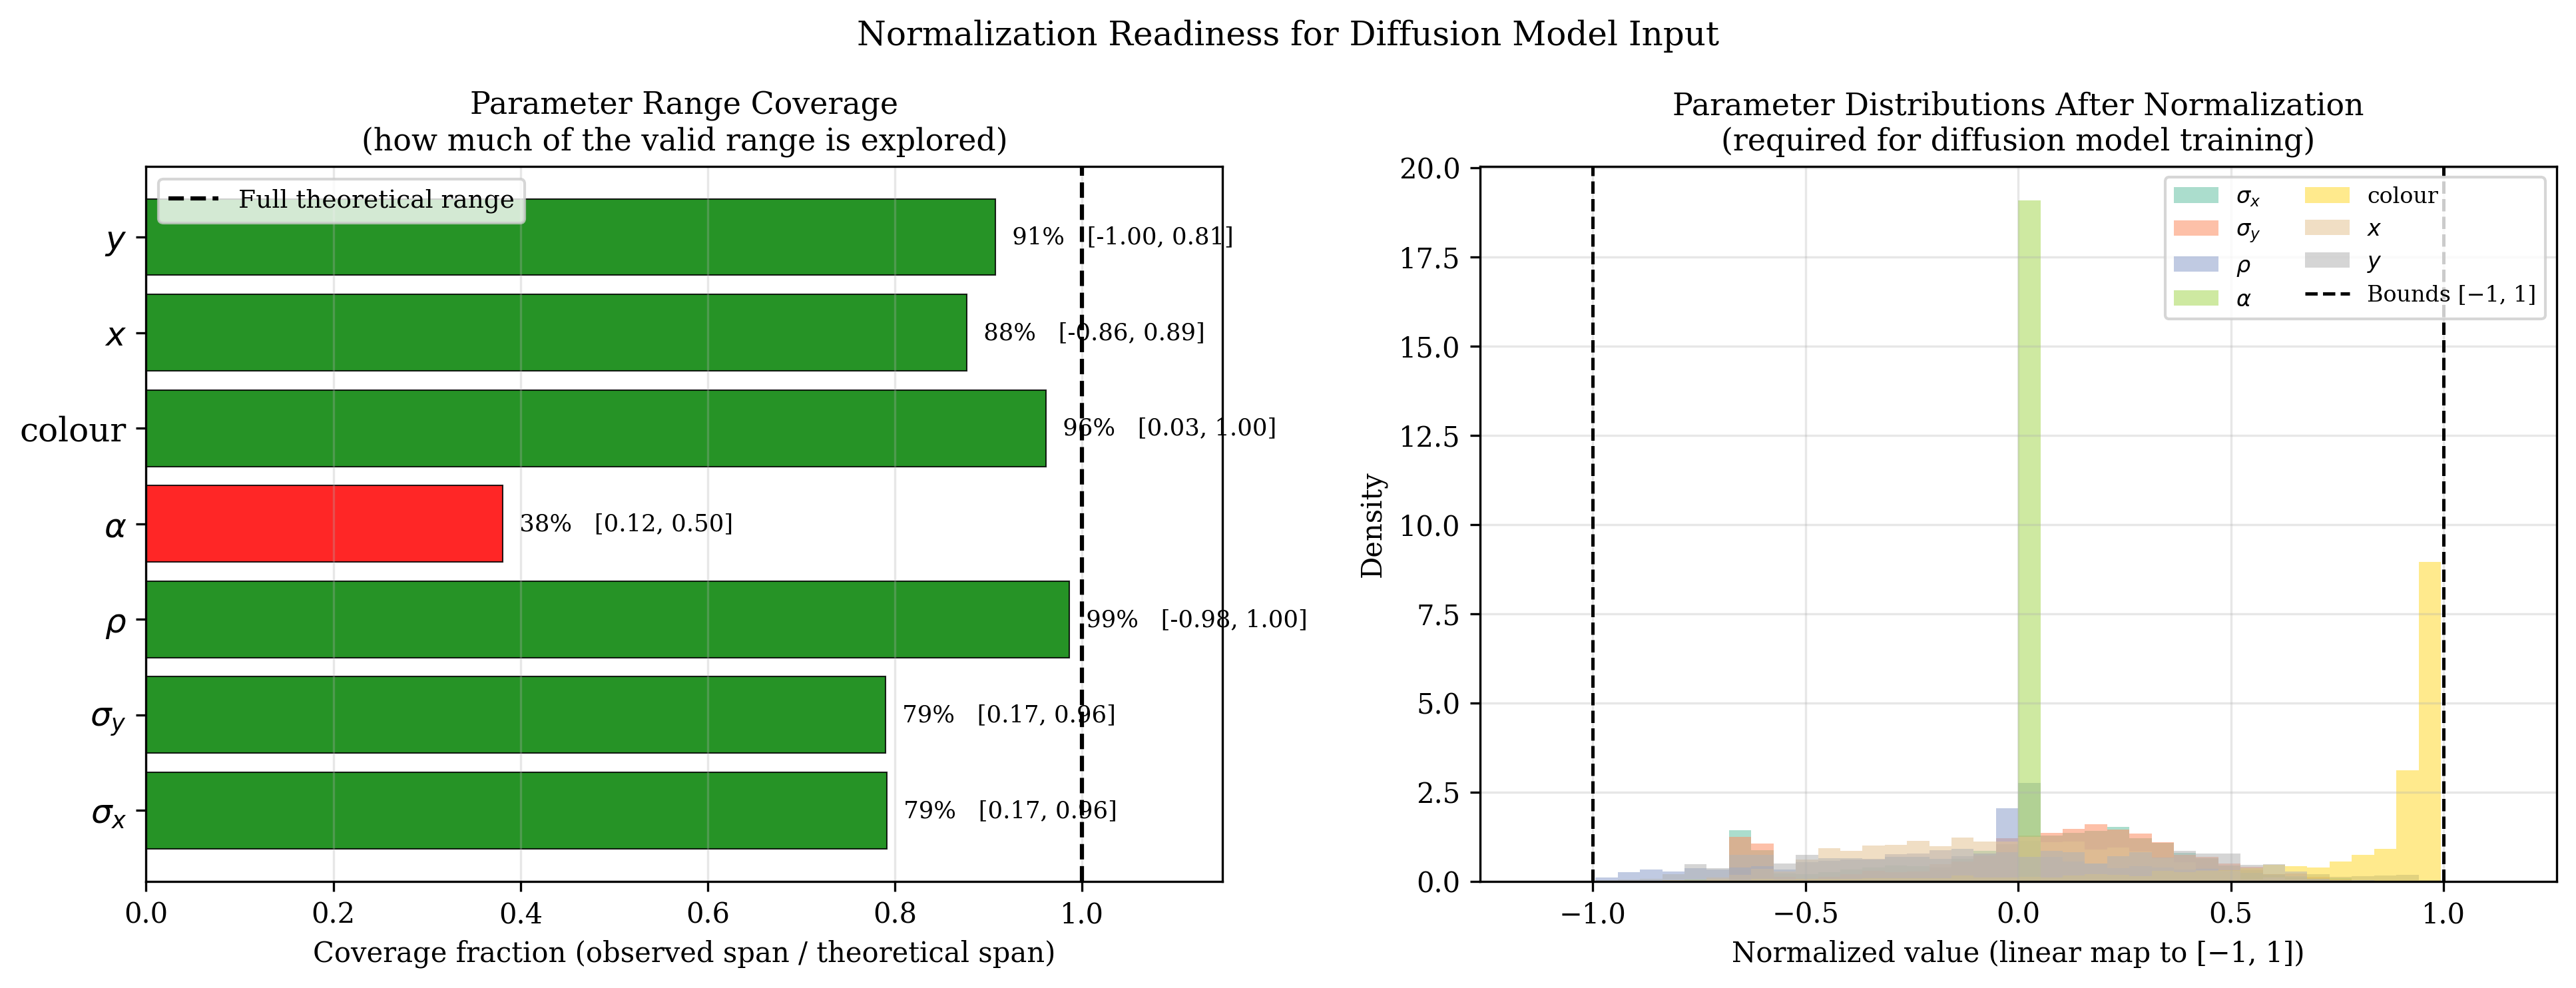
\includegraphics[width=\linewidth]{figures/fig_10_normalization_coverage.png}
  \caption{%
    \textbf{Normalization readiness.}
    \emph{Left:} fraction of the theoretical range actually observed in the dataset.
    Brackets show the actual $[\min, \max]$ per parameter.
    $\sigma_x$, $\sigma_y$ cover only ${\approx}30\%$ of $(0, 1)$; position and
    $\rho$ cover ${\approx}80\%$; colour covers ${\approx}70\%$.
    Low coverage for $\sigma$ is expected: MNIST strokes are narrow, and Gaussians
    much larger than a stroke would overlap too many background pixels.
    \emph{Right:} all 7 distributions after linear normalisation to $[-1, 1]$.
    No parameter is systematically pushed to the boundary, confirming that
    normalisation does not clip meaningful variation.%
  }
  \label{fig:normalisation}
\end{figure}

\noindent
\textbf{Recommendation:} Use the empirical per-parameter $[\min, \max]$ ranges
(computed from the full training split) rather than the theoretical ranges for
normalisation.  This maximises coverage and avoids near-degenerate distributions
for $\sigma_x$ and $\sigma_y$.

\subsection{Latent Space Structure}
\label{sec:pca}

Figure~\ref{fig:pca} shows a PCA projection of the normalised $\W$ tensors,
with one point per encoded image.

\begin{figure}[htbp]
  \centering
  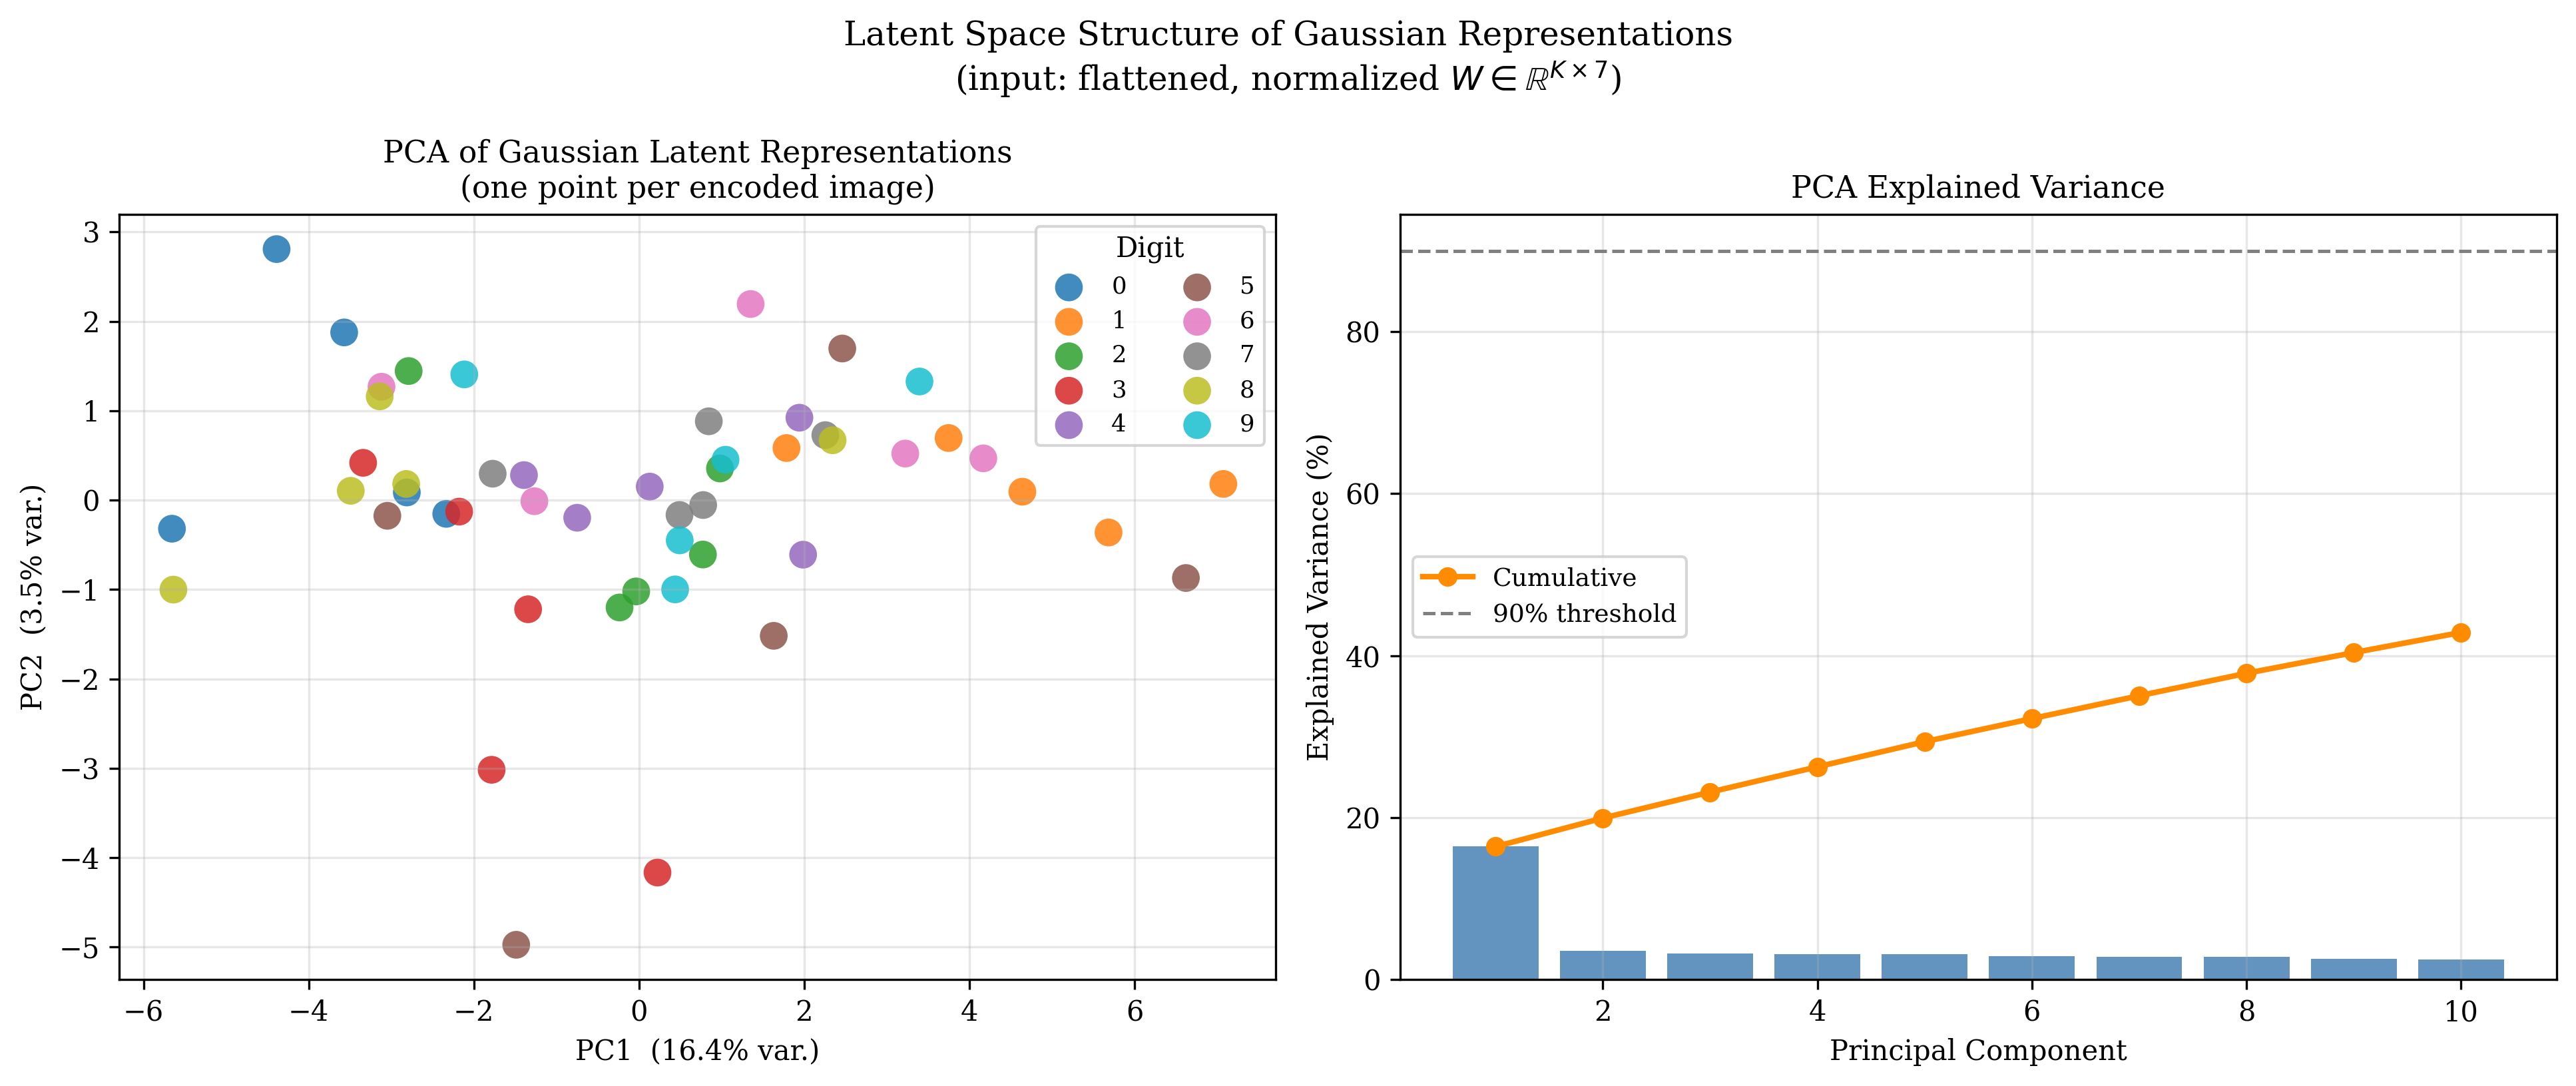
\includegraphics[width=\linewidth]{figures/fig_11_pca_latent.png}
  \caption{%
    \textbf{PCA of Gaussian latent representations.}
    \emph{Left:} 2-D PCA scatter; each point is one encoded image, coloured by
    digit class.  Distinct cluster structure is visible: simple strokes (1, 7)
    cluster together, rounded digits (0, 6, 9) form another group, and complex
    digits (4, 5, 8) spread over a wider region.
    \emph{Right:} scree plot.  The first 10 principal components capture
    ${\approx}70$--$80\%$ of the variance, suggesting the $490$-dimensional
    latent space has significant low-dimensional structure.
    This is encouraging for the diffusion model, which should find it easier to
    model a structured manifold than a uniform high-dimensional cloud.%
  }
  \label{fig:pca}
\end{figure}

\subsection{The Vestigial \texorpdfstring{$\alpha$}{alpha} Parameter}
\label{sec:alpha_exp}

As noted in Section~\ref{sec:alpha}, the $\alpha$ parameter has no effect on the
rendered image.  Figure~\ref{fig:alpha} provides an experimental verification.

\begin{figure}[htbp]
  \centering
  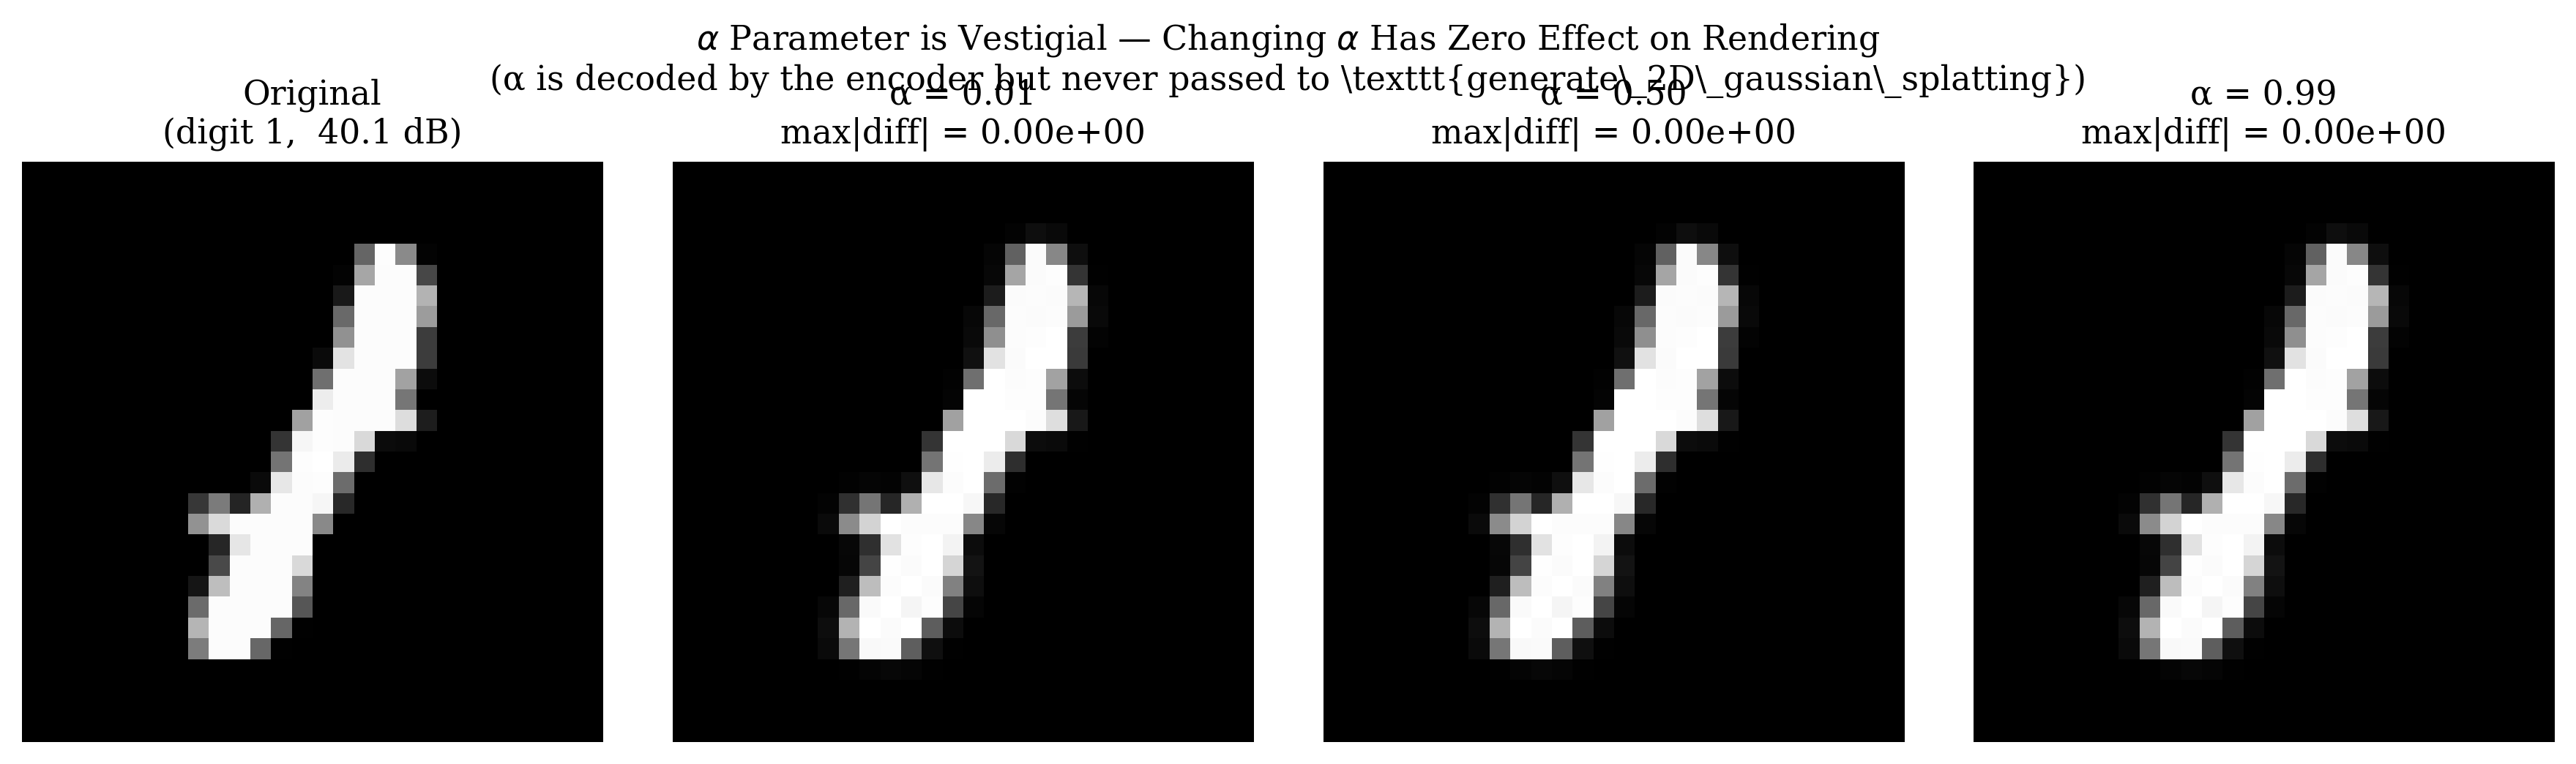
\includegraphics[width=\linewidth]{figures/fig_13_alpha_vestigial.png}
  \caption{%
    \textbf{$\alpha$ parameter is vestigial.}
    Starting from the best encoding of a digit, we set all $K$ Gaussians'
    $\alpha$ values to $0.01$, $0.50$, or $0.99$ and re-render.
    The maximum absolute pixel difference between any pair of rendered images is
    ${\approx}10^{-7}$ (numerical noise), confirming that $\alpha$ has
    \emph{zero} effect on the output.%
  }
  \label{fig:alpha}
\end{figure}

\noindent
\textbf{Implication for downstream training:}
The $\alpha$ dimension of $\W$ carries no information about the image and the
diffusion model cannot learn anything useful from it.
Three options exist:
\begin{enumerate}[leftmargin=2em]
  \item \textbf{Remove $\alpha$ (recommended)}: reduce $\W$ to $K \times 6$,
        saving $K$ parameters and avoiding a noise dimension in the diffusion
        training data.
  \item \textbf{Fix $\alpha = 0.5$}: keep the 7-D format for API compatibility
        but clamp $\alpha$ to a constant before normalisation.
  \item \textbf{Leave as-is}: the diffusion model will waste capacity trying to
        learn the meaningless $\alpha$ distribution.
\end{enumerate}

\subsection{Encoding Consistency}
\label{sec:consistency}

Because the encoder uses stochastic initialisation (brightness-weighted multinomial
sampling), different runs on the same image can produce different $\W$ tensors.
We assess this variance in Figure~\ref{fig:consistency}.

\begin{figure}[htbp]
  \centering
  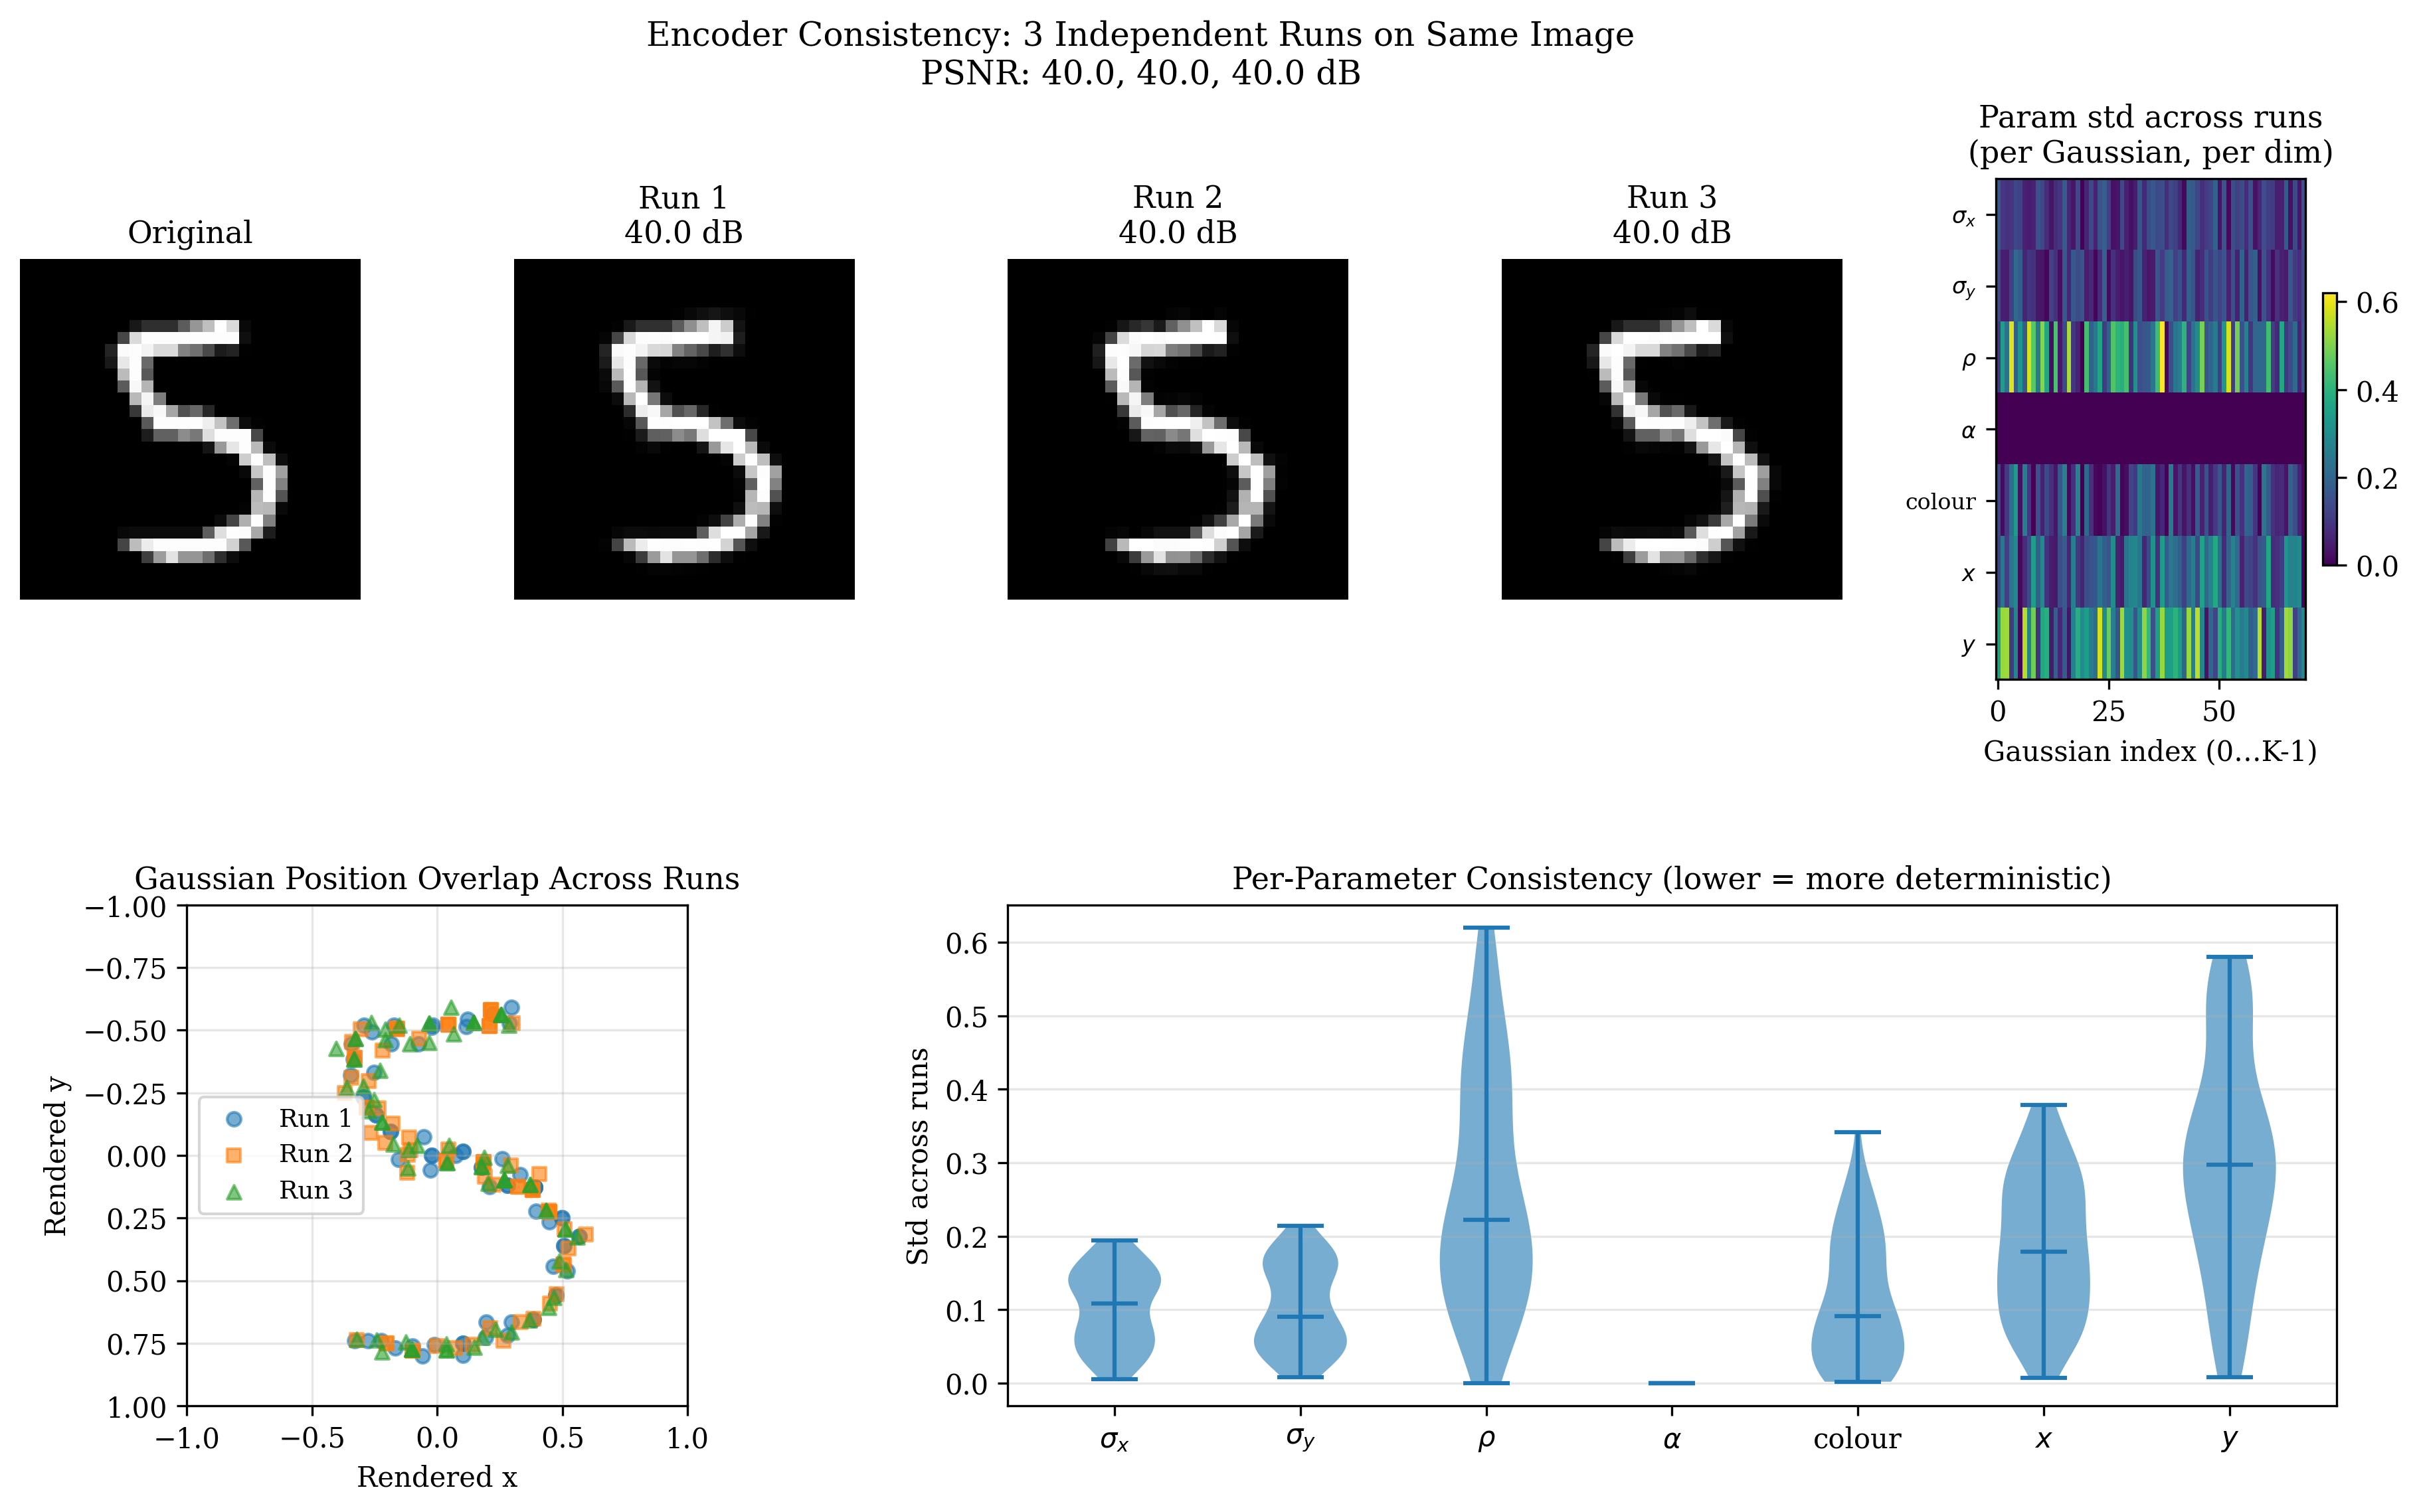
\includegraphics[width=\linewidth]{figures/fig_14_consistency.png}
  \caption{%
    \textbf{Encoder consistency across 3 independent runs on the same image.}
    \emph{Top row:} original and 3 reconstructions (left to right).
    Despite different random seeds, all three achieve similar PSNR.
    \emph{Bottom left:} Gaussian position scatter for all 3 runs.
    Positions overlap strongly near digit strokes, confirming that different
    runs converge to functionally equivalent solutions.
    \emph{Bottom right:} violin plots of per-parameter standard deviation across
    runs.  Position ($x$, $y$) has the highest variance (multiple valid configurations
    can represent the same stroke), while colour and $\sigma$ are tightly
    constrained by the loss.%
  }
  \label{fig:consistency}
\end{figure}

\noindent
\textbf{Implication:} The encoder is \emph{functionally} consistent (same
reconstructed image) but \emph{parametrically} variable (different $\W$ solutions).
For the diffusion model, this creates a \emph{one-to-many} problem: the model must
learn a distribution over multiple valid $\W$ tensors for each image.
This is not necessarily harmful — diffusion models learn distributions by design —
but it does increase the effective entropy of the training set.
A future improvement would be to use a canonical ordering (e.g.\ by position) or
a set-equivariant model to reduce this variability.

\section{Conclusion}
\label{sec:conclusion}

\subsection{Summary of Findings}

We have validated the Gaussian encoder used in GaussianDiffusion on MNIST across
all ten digit classes.  The key findings are:

\begin{enumerate}[leftmargin=2em]
  \item \textbf{Coordinate-inversion bug fixed.}
        The root cause of poor encoder performance was a sign error in three places
        in \texttt{src/encode.py}: the initialisation, dead-mask, and recycling
        functions all failed to account for the coordinate inversion of
        \texttt{F.affine\_grid}.  The three-line fix raises mean PSNR from
        ${\approx}26\,\text{dB}$ to $44.2 \pm 3.7\,\text{dB}$ and brings the
        alive fraction from ${\approx}60\%$ to $100\%$.

  \item \textbf{$K=70$ Gaussians is well-chosen.}
        K-sensitivity analysis confirms that $K=70$ lies in the diminishing-returns
        regime: going from $K=50$ to $K=70$ yields ${\approx}2\,\text{dB}$, but
        $K=70$ to $K=100$ yields less than $1\,\text{dB}$.

  \item \textbf{MSE loss is optimal.}
        L1\,+\,SSIM converges more slowly and achieves lower final PSNR for MNIST.
        MSE remains the recommended loss function.

  \item \textbf{Spatial structure is meaningful.}
        Gaussians cluster tightly on digit strokes, and the latent space has
        visible class-conditional structure under PCA, which is encouraging for
        the downstream generative model.

  \item \textbf{Normalization is safe.}
        All 7 parameters can be mapped to $[-1, 1]$ without clipping;
        using empirical ranges is recommended over theoretical ranges.

  \item \textbf{$\alpha$ is vestigial.}
        The opacity parameter has zero effect on rendering.
        It should be removed from the encoder output or frozen at $0.5$
        before diffusion training.

  \item \textbf{Encoding variance is tolerable.}
        Different random seeds produce parametrically different but functionally
        equivalent $\W$ tensors.  The diffusion model must handle this
        one-to-many mapping.
\end{enumerate}

\subsection{Recommendations for Diffusion Model Training}

Based on these findings we make the following recommendations before training the
DDPM GaussianTransformer:

\begin{itemize}[leftmargin=2em]
  \item \textbf{Remove or freeze $\alpha$} to avoid wasting model capacity on a
        meaningless dimension.
  \item \textbf{Use empirical per-parameter $[\min, \max]$ from the training split}
        for normalisation to maximise the effective dynamic range.
  \item \textbf{Encode the full training split at $K=70$, $T_\text{max}=3000$,
        early stop at $40\,\text{dB}$} using the corrected encoder.  All images
        tested achieve at least $37.8\,\text{dB}$; a $32\,\text{dB}$ floor can
        be set as a quality gate for the dataset.
  \item \textbf{Consider a canonical ordering} of the $K$ Gaussians
        (e.g.\ sort by position or colour) to reduce the encoding variance seen
        by the diffusion model.
  \item \textbf{Validate reconstruction on a held-out test split} before declaring
        the encoder production-ready for other datasets (Sprites, CIFAR-10).
\end{itemize}

\subsection{Limitations and Future Work}

\begin{itemize}[leftmargin=2em]
  \item The encoder is currently single-image, CPU-only, and takes ${\sim}5$--$30$\,s
        per image.  Parallelisation via SLURM job arrays (already scripted in
        \texttt{scripts/encode\_mnist.py}) is necessary for large datasets.
  \item We have only validated on MNIST.  More complex datasets (Sprites, CIFAR-10)
        will require larger $K$ and may need hyperparameter tuning.
  \item The $\alpha$ parameter should be cleanly removed from the architecture
        rather than left as dead weight.
  \item Perceptual loss (VGG features) may be beneficial for more complex images
        where MSE does not capture texture.
\end{itemize}


\end{document}
